
% Default to the notebook output style

    


% Inherit from the specified cell style.




    
\documentclass[11pt]{article}

    
    
    \usepackage[T1]{fontenc}
    % Nicer default font (+ math font) than Computer Modern for most use cases
    \usepackage{mathpazo}

    % Basic figure setup, for now with no caption control since it's done
    % automatically by Pandoc (which extracts ![](path) syntax from Markdown).
    \usepackage{graphicx}
    % We will generate all images so they have a width \maxwidth. This means
    % that they will get their normal width if they fit onto the page, but
    % are scaled down if they would overflow the margins.
    \makeatletter
    \def\maxwidth{\ifdim\Gin@nat@width>\linewidth\linewidth
    \else\Gin@nat@width\fi}
    \makeatother
    \let\Oldincludegraphics\includegraphics
    % Set max figure width to be 80% of text width, for now hardcoded.
    \renewcommand{\includegraphics}[1]{\Oldincludegraphics[width=.8\maxwidth]{#1}}
    % Ensure that by default, figures have no caption (until we provide a
    % proper Figure object with a Caption API and a way to capture that
    % in the conversion process - todo).
    \usepackage{caption}
    \DeclareCaptionLabelFormat{nolabel}{}
    \captionsetup{labelformat=nolabel}

    \usepackage{adjustbox} % Used to constrain images to a maximum size 
    \usepackage{xcolor} % Allow colors to be defined
    \usepackage{enumerate} % Needed for markdown enumerations to work
    \usepackage{geometry} % Used to adjust the document margins
    \usepackage{amsmath} % Equations
    \usepackage{amssymb} % Equations
    \usepackage{textcomp} % defines textquotesingle
    % Hack from http://tex.stackexchange.com/a/47451/13684:
    \AtBeginDocument{%
        \def\PYZsq{\textquotesingle}% Upright quotes in Pygmentized code
    }
    \usepackage{upquote} % Upright quotes for verbatim code
    \usepackage{eurosym} % defines \euro
    \usepackage[mathletters]{ucs} % Extended unicode (utf-8) support
    \usepackage[utf8x]{inputenc} % Allow utf-8 characters in the tex document
    \usepackage{fancyvrb} % verbatim replacement that allows latex
    \usepackage{grffile} % extends the file name processing of package graphics 
                         % to support a larger range 
    % The hyperref package gives us a pdf with properly built
    % internal navigation ('pdf bookmarks' for the table of contents,
    % internal cross-reference links, web links for URLs, etc.)
    \usepackage{hyperref}
    \usepackage{longtable} % longtable support required by pandoc >1.10
    \usepackage{booktabs}  % table support for pandoc > 1.12.2
    \usepackage[inline]{enumitem} % IRkernel/repr support (it uses the enumerate* environment)
    \usepackage[normalem]{ulem} % ulem is needed to support strikethroughs (\sout)
                                % normalem makes italics be italics, not underlines
    

    
    
    % Colors for the hyperref package
    \definecolor{urlcolor}{rgb}{0,.145,.698}
    \definecolor{linkcolor}{rgb}{.71,0.21,0.01}
    \definecolor{citecolor}{rgb}{.12,.54,.11}

    % ANSI colors
    \definecolor{ansi-black}{HTML}{3E424D}
    \definecolor{ansi-black-intense}{HTML}{282C36}
    \definecolor{ansi-red}{HTML}{E75C58}
    \definecolor{ansi-red-intense}{HTML}{B22B31}
    \definecolor{ansi-green}{HTML}{00A250}
    \definecolor{ansi-green-intense}{HTML}{007427}
    \definecolor{ansi-yellow}{HTML}{DDB62B}
    \definecolor{ansi-yellow-intense}{HTML}{B27D12}
    \definecolor{ansi-blue}{HTML}{208FFB}
    \definecolor{ansi-blue-intense}{HTML}{0065CA}
    \definecolor{ansi-magenta}{HTML}{D160C4}
    \definecolor{ansi-magenta-intense}{HTML}{A03196}
    \definecolor{ansi-cyan}{HTML}{60C6C8}
    \definecolor{ansi-cyan-intense}{HTML}{258F8F}
    \definecolor{ansi-white}{HTML}{C5C1B4}
    \definecolor{ansi-white-intense}{HTML}{A1A6B2}

    % commands and environments needed by pandoc snippets
    % extracted from the output of `pandoc -s`
    \providecommand{\tightlist}{%
      \setlength{\itemsep}{0pt}\setlength{\parskip}{0pt}}
    \DefineVerbatimEnvironment{Highlighting}{Verbatim}{commandchars=\\\{\}}
    % Add ',fontsize=\small' for more characters per line
    \newenvironment{Shaded}{}{}
    \newcommand{\KeywordTok}[1]{\textcolor[rgb]{0.00,0.44,0.13}{\textbf{{#1}}}}
    \newcommand{\DataTypeTok}[1]{\textcolor[rgb]{0.56,0.13,0.00}{{#1}}}
    \newcommand{\DecValTok}[1]{\textcolor[rgb]{0.25,0.63,0.44}{{#1}}}
    \newcommand{\BaseNTok}[1]{\textcolor[rgb]{0.25,0.63,0.44}{{#1}}}
    \newcommand{\FloatTok}[1]{\textcolor[rgb]{0.25,0.63,0.44}{{#1}}}
    \newcommand{\CharTok}[1]{\textcolor[rgb]{0.25,0.44,0.63}{{#1}}}
    \newcommand{\StringTok}[1]{\textcolor[rgb]{0.25,0.44,0.63}{{#1}}}
    \newcommand{\CommentTok}[1]{\textcolor[rgb]{0.38,0.63,0.69}{\textit{{#1}}}}
    \newcommand{\OtherTok}[1]{\textcolor[rgb]{0.00,0.44,0.13}{{#1}}}
    \newcommand{\AlertTok}[1]{\textcolor[rgb]{1.00,0.00,0.00}{\textbf{{#1}}}}
    \newcommand{\FunctionTok}[1]{\textcolor[rgb]{0.02,0.16,0.49}{{#1}}}
    \newcommand{\RegionMarkerTok}[1]{{#1}}
    \newcommand{\ErrorTok}[1]{\textcolor[rgb]{1.00,0.00,0.00}{\textbf{{#1}}}}
    \newcommand{\NormalTok}[1]{{#1}}
    
    % Additional commands for more recent versions of Pandoc
    \newcommand{\ConstantTok}[1]{\textcolor[rgb]{0.53,0.00,0.00}{{#1}}}
    \newcommand{\SpecialCharTok}[1]{\textcolor[rgb]{0.25,0.44,0.63}{{#1}}}
    \newcommand{\VerbatimStringTok}[1]{\textcolor[rgb]{0.25,0.44,0.63}{{#1}}}
    \newcommand{\SpecialStringTok}[1]{\textcolor[rgb]{0.73,0.40,0.53}{{#1}}}
    \newcommand{\ImportTok}[1]{{#1}}
    \newcommand{\DocumentationTok}[1]{\textcolor[rgb]{0.73,0.13,0.13}{\textit{{#1}}}}
    \newcommand{\AnnotationTok}[1]{\textcolor[rgb]{0.38,0.63,0.69}{\textbf{\textit{{#1}}}}}
    \newcommand{\CommentVarTok}[1]{\textcolor[rgb]{0.38,0.63,0.69}{\textbf{\textit{{#1}}}}}
    \newcommand{\VariableTok}[1]{\textcolor[rgb]{0.10,0.09,0.49}{{#1}}}
    \newcommand{\ControlFlowTok}[1]{\textcolor[rgb]{0.00,0.44,0.13}{\textbf{{#1}}}}
    \newcommand{\OperatorTok}[1]{\textcolor[rgb]{0.40,0.40,0.40}{{#1}}}
    \newcommand{\BuiltInTok}[1]{{#1}}
    \newcommand{\ExtensionTok}[1]{{#1}}
    \newcommand{\PreprocessorTok}[1]{\textcolor[rgb]{0.74,0.48,0.00}{{#1}}}
    \newcommand{\AttributeTok}[1]{\textcolor[rgb]{0.49,0.56,0.16}{{#1}}}
    \newcommand{\InformationTok}[1]{\textcolor[rgb]{0.38,0.63,0.69}{\textbf{\textit{{#1}}}}}
    \newcommand{\WarningTok}[1]{\textcolor[rgb]{0.38,0.63,0.69}{\textbf{\textit{{#1}}}}}
    
    
    % Define a nice break command that doesn't care if a line doesn't already
    % exist.
    \def\br{\hspace*{\fill} \\* }
    % Math Jax compatability definitions
    \def\gt{>}
    \def\lt{<}
    % Document parameters
    \title{P3 Image Denoising}
    
    
    

    % Pygments definitions
    
\makeatletter
\def\PY@reset{\let\PY@it=\relax \let\PY@bf=\relax%
    \let\PY@ul=\relax \let\PY@tc=\relax%
    \let\PY@bc=\relax \let\PY@ff=\relax}
\def\PY@tok#1{\csname PY@tok@#1\endcsname}
\def\PY@toks#1+{\ifx\relax#1\empty\else%
    \PY@tok{#1}\expandafter\PY@toks\fi}
\def\PY@do#1{\PY@bc{\PY@tc{\PY@ul{%
    \PY@it{\PY@bf{\PY@ff{#1}}}}}}}
\def\PY#1#2{\PY@reset\PY@toks#1+\relax+\PY@do{#2}}

\expandafter\def\csname PY@tok@w\endcsname{\def\PY@tc##1{\textcolor[rgb]{0.73,0.73,0.73}{##1}}}
\expandafter\def\csname PY@tok@c\endcsname{\let\PY@it=\textit\def\PY@tc##1{\textcolor[rgb]{0.25,0.50,0.50}{##1}}}
\expandafter\def\csname PY@tok@cp\endcsname{\def\PY@tc##1{\textcolor[rgb]{0.74,0.48,0.00}{##1}}}
\expandafter\def\csname PY@tok@k\endcsname{\let\PY@bf=\textbf\def\PY@tc##1{\textcolor[rgb]{0.00,0.50,0.00}{##1}}}
\expandafter\def\csname PY@tok@kp\endcsname{\def\PY@tc##1{\textcolor[rgb]{0.00,0.50,0.00}{##1}}}
\expandafter\def\csname PY@tok@kt\endcsname{\def\PY@tc##1{\textcolor[rgb]{0.69,0.00,0.25}{##1}}}
\expandafter\def\csname PY@tok@o\endcsname{\def\PY@tc##1{\textcolor[rgb]{0.40,0.40,0.40}{##1}}}
\expandafter\def\csname PY@tok@ow\endcsname{\let\PY@bf=\textbf\def\PY@tc##1{\textcolor[rgb]{0.67,0.13,1.00}{##1}}}
\expandafter\def\csname PY@tok@nb\endcsname{\def\PY@tc##1{\textcolor[rgb]{0.00,0.50,0.00}{##1}}}
\expandafter\def\csname PY@tok@nf\endcsname{\def\PY@tc##1{\textcolor[rgb]{0.00,0.00,1.00}{##1}}}
\expandafter\def\csname PY@tok@nc\endcsname{\let\PY@bf=\textbf\def\PY@tc##1{\textcolor[rgb]{0.00,0.00,1.00}{##1}}}
\expandafter\def\csname PY@tok@nn\endcsname{\let\PY@bf=\textbf\def\PY@tc##1{\textcolor[rgb]{0.00,0.00,1.00}{##1}}}
\expandafter\def\csname PY@tok@ne\endcsname{\let\PY@bf=\textbf\def\PY@tc##1{\textcolor[rgb]{0.82,0.25,0.23}{##1}}}
\expandafter\def\csname PY@tok@nv\endcsname{\def\PY@tc##1{\textcolor[rgb]{0.10,0.09,0.49}{##1}}}
\expandafter\def\csname PY@tok@no\endcsname{\def\PY@tc##1{\textcolor[rgb]{0.53,0.00,0.00}{##1}}}
\expandafter\def\csname PY@tok@nl\endcsname{\def\PY@tc##1{\textcolor[rgb]{0.63,0.63,0.00}{##1}}}
\expandafter\def\csname PY@tok@ni\endcsname{\let\PY@bf=\textbf\def\PY@tc##1{\textcolor[rgb]{0.60,0.60,0.60}{##1}}}
\expandafter\def\csname PY@tok@na\endcsname{\def\PY@tc##1{\textcolor[rgb]{0.49,0.56,0.16}{##1}}}
\expandafter\def\csname PY@tok@nt\endcsname{\let\PY@bf=\textbf\def\PY@tc##1{\textcolor[rgb]{0.00,0.50,0.00}{##1}}}
\expandafter\def\csname PY@tok@nd\endcsname{\def\PY@tc##1{\textcolor[rgb]{0.67,0.13,1.00}{##1}}}
\expandafter\def\csname PY@tok@s\endcsname{\def\PY@tc##1{\textcolor[rgb]{0.73,0.13,0.13}{##1}}}
\expandafter\def\csname PY@tok@sd\endcsname{\let\PY@it=\textit\def\PY@tc##1{\textcolor[rgb]{0.73,0.13,0.13}{##1}}}
\expandafter\def\csname PY@tok@si\endcsname{\let\PY@bf=\textbf\def\PY@tc##1{\textcolor[rgb]{0.73,0.40,0.53}{##1}}}
\expandafter\def\csname PY@tok@se\endcsname{\let\PY@bf=\textbf\def\PY@tc##1{\textcolor[rgb]{0.73,0.40,0.13}{##1}}}
\expandafter\def\csname PY@tok@sr\endcsname{\def\PY@tc##1{\textcolor[rgb]{0.73,0.40,0.53}{##1}}}
\expandafter\def\csname PY@tok@ss\endcsname{\def\PY@tc##1{\textcolor[rgb]{0.10,0.09,0.49}{##1}}}
\expandafter\def\csname PY@tok@sx\endcsname{\def\PY@tc##1{\textcolor[rgb]{0.00,0.50,0.00}{##1}}}
\expandafter\def\csname PY@tok@m\endcsname{\def\PY@tc##1{\textcolor[rgb]{0.40,0.40,0.40}{##1}}}
\expandafter\def\csname PY@tok@gh\endcsname{\let\PY@bf=\textbf\def\PY@tc##1{\textcolor[rgb]{0.00,0.00,0.50}{##1}}}
\expandafter\def\csname PY@tok@gu\endcsname{\let\PY@bf=\textbf\def\PY@tc##1{\textcolor[rgb]{0.50,0.00,0.50}{##1}}}
\expandafter\def\csname PY@tok@gd\endcsname{\def\PY@tc##1{\textcolor[rgb]{0.63,0.00,0.00}{##1}}}
\expandafter\def\csname PY@tok@gi\endcsname{\def\PY@tc##1{\textcolor[rgb]{0.00,0.63,0.00}{##1}}}
\expandafter\def\csname PY@tok@gr\endcsname{\def\PY@tc##1{\textcolor[rgb]{1.00,0.00,0.00}{##1}}}
\expandafter\def\csname PY@tok@ge\endcsname{\let\PY@it=\textit}
\expandafter\def\csname PY@tok@gs\endcsname{\let\PY@bf=\textbf}
\expandafter\def\csname PY@tok@gp\endcsname{\let\PY@bf=\textbf\def\PY@tc##1{\textcolor[rgb]{0.00,0.00,0.50}{##1}}}
\expandafter\def\csname PY@tok@go\endcsname{\def\PY@tc##1{\textcolor[rgb]{0.53,0.53,0.53}{##1}}}
\expandafter\def\csname PY@tok@gt\endcsname{\def\PY@tc##1{\textcolor[rgb]{0.00,0.27,0.87}{##1}}}
\expandafter\def\csname PY@tok@err\endcsname{\def\PY@bc##1{\setlength{\fboxsep}{0pt}\fcolorbox[rgb]{1.00,0.00,0.00}{1,1,1}{\strut ##1}}}
\expandafter\def\csname PY@tok@kc\endcsname{\let\PY@bf=\textbf\def\PY@tc##1{\textcolor[rgb]{0.00,0.50,0.00}{##1}}}
\expandafter\def\csname PY@tok@kd\endcsname{\let\PY@bf=\textbf\def\PY@tc##1{\textcolor[rgb]{0.00,0.50,0.00}{##1}}}
\expandafter\def\csname PY@tok@kn\endcsname{\let\PY@bf=\textbf\def\PY@tc##1{\textcolor[rgb]{0.00,0.50,0.00}{##1}}}
\expandafter\def\csname PY@tok@kr\endcsname{\let\PY@bf=\textbf\def\PY@tc##1{\textcolor[rgb]{0.00,0.50,0.00}{##1}}}
\expandafter\def\csname PY@tok@bp\endcsname{\def\PY@tc##1{\textcolor[rgb]{0.00,0.50,0.00}{##1}}}
\expandafter\def\csname PY@tok@fm\endcsname{\def\PY@tc##1{\textcolor[rgb]{0.00,0.00,1.00}{##1}}}
\expandafter\def\csname PY@tok@vc\endcsname{\def\PY@tc##1{\textcolor[rgb]{0.10,0.09,0.49}{##1}}}
\expandafter\def\csname PY@tok@vg\endcsname{\def\PY@tc##1{\textcolor[rgb]{0.10,0.09,0.49}{##1}}}
\expandafter\def\csname PY@tok@vi\endcsname{\def\PY@tc##1{\textcolor[rgb]{0.10,0.09,0.49}{##1}}}
\expandafter\def\csname PY@tok@vm\endcsname{\def\PY@tc##1{\textcolor[rgb]{0.10,0.09,0.49}{##1}}}
\expandafter\def\csname PY@tok@sa\endcsname{\def\PY@tc##1{\textcolor[rgb]{0.73,0.13,0.13}{##1}}}
\expandafter\def\csname PY@tok@sb\endcsname{\def\PY@tc##1{\textcolor[rgb]{0.73,0.13,0.13}{##1}}}
\expandafter\def\csname PY@tok@sc\endcsname{\def\PY@tc##1{\textcolor[rgb]{0.73,0.13,0.13}{##1}}}
\expandafter\def\csname PY@tok@dl\endcsname{\def\PY@tc##1{\textcolor[rgb]{0.73,0.13,0.13}{##1}}}
\expandafter\def\csname PY@tok@s2\endcsname{\def\PY@tc##1{\textcolor[rgb]{0.73,0.13,0.13}{##1}}}
\expandafter\def\csname PY@tok@sh\endcsname{\def\PY@tc##1{\textcolor[rgb]{0.73,0.13,0.13}{##1}}}
\expandafter\def\csname PY@tok@s1\endcsname{\def\PY@tc##1{\textcolor[rgb]{0.73,0.13,0.13}{##1}}}
\expandafter\def\csname PY@tok@mb\endcsname{\def\PY@tc##1{\textcolor[rgb]{0.40,0.40,0.40}{##1}}}
\expandafter\def\csname PY@tok@mf\endcsname{\def\PY@tc##1{\textcolor[rgb]{0.40,0.40,0.40}{##1}}}
\expandafter\def\csname PY@tok@mh\endcsname{\def\PY@tc##1{\textcolor[rgb]{0.40,0.40,0.40}{##1}}}
\expandafter\def\csname PY@tok@mi\endcsname{\def\PY@tc##1{\textcolor[rgb]{0.40,0.40,0.40}{##1}}}
\expandafter\def\csname PY@tok@il\endcsname{\def\PY@tc##1{\textcolor[rgb]{0.40,0.40,0.40}{##1}}}
\expandafter\def\csname PY@tok@mo\endcsname{\def\PY@tc##1{\textcolor[rgb]{0.40,0.40,0.40}{##1}}}
\expandafter\def\csname PY@tok@ch\endcsname{\let\PY@it=\textit\def\PY@tc##1{\textcolor[rgb]{0.25,0.50,0.50}{##1}}}
\expandafter\def\csname PY@tok@cm\endcsname{\let\PY@it=\textit\def\PY@tc##1{\textcolor[rgb]{0.25,0.50,0.50}{##1}}}
\expandafter\def\csname PY@tok@cpf\endcsname{\let\PY@it=\textit\def\PY@tc##1{\textcolor[rgb]{0.25,0.50,0.50}{##1}}}
\expandafter\def\csname PY@tok@c1\endcsname{\let\PY@it=\textit\def\PY@tc##1{\textcolor[rgb]{0.25,0.50,0.50}{##1}}}
\expandafter\def\csname PY@tok@cs\endcsname{\let\PY@it=\textit\def\PY@tc##1{\textcolor[rgb]{0.25,0.50,0.50}{##1}}}

\def\PYZbs{\char`\\}
\def\PYZus{\char`\_}
\def\PYZob{\char`\{}
\def\PYZcb{\char`\}}
\def\PYZca{\char`\^}
\def\PYZam{\char`\&}
\def\PYZlt{\char`\<}
\def\PYZgt{\char`\>}
\def\PYZsh{\char`\#}
\def\PYZpc{\char`\%}
\def\PYZdl{\char`\$}
\def\PYZhy{\char`\-}
\def\PYZsq{\char`\'}
\def\PYZdq{\char`\"}
\def\PYZti{\char`\~}
% for compatibility with earlier versions
\def\PYZat{@}
\def\PYZlb{[}
\def\PYZrb{]}
\makeatother


    % Exact colors from NB
    \definecolor{incolor}{rgb}{0.0, 0.0, 0.5}
    \definecolor{outcolor}{rgb}{0.545, 0.0, 0.0}



    
    % Prevent overflowing lines due to hard-to-break entities
    \sloppy 
    % Setup hyperref package
    \hypersetup{
      breaklinks=true,  % so long urls are correctly broken across lines
      colorlinks=true,
      urlcolor=urlcolor,
      linkcolor=linkcolor,
      citecolor=citecolor,
      }
    % Slightly bigger margins than the latex defaults
    
    \geometry{verbose,tmargin=1in,bmargin=1in,lmargin=1in,rmargin=1in}
    
    

    \begin{document}
    
    
    \maketitle
    
    

    
    \hypertarget{p3-image-denoising}{%
\section{P3 Image Denoising}\label{p3-image-denoising}}

    \hypertarget{will-koehrsen-wjk68}{%
\subsection{Will Koehrsen wjk68}\label{will-koehrsen-wjk68}}

    \hypertarget{problem-explanation}{%
\section{Problem Explanation}\label{problem-explanation}}

In this notebook, we will the concepted of undirected graphs to remove
noise from a binary image of 0s and 1s. The noisy image itself forms the
observed variables, \(y_i \in \{−1, +1\}\), and the hidden variables are
the true image, that is the image without any noise,
\(x_i \in \{−1, +1\}\).

We assume that the noisy image is created by randomly flipping a small
percentage of the bits in the original image. We can then use an energy
function and the concept of cliques between adjacent pixels to flip the
values of the noisy image to reduce the total energy value. There should
be a correlation both between neighboring pixels in the noisy image,
\(x_i\) and \(x_j\) and between pixels in the noisy image \(x_i\) and
hidden, noise-free image \(y_i\). The two types of cliques in the image
are thus \(\{x_i, x_j\}\) between neighboring pixels, and
\(\{x_i, y_i\}\) between pixels in the observed and hidden images.
Further explanation of the energy function appears later in the
notebook.

    \begin{Verbatim}[commandchars=\\\{\}]
{\color{incolor}In [{\color{incolor}1}]:} \PY{k+kn}{import} \PY{n+nn}{pandas} \PY{k}{as} \PY{n+nn}{pd}
        \PY{k+kn}{import} \PY{n+nn}{numpy} \PY{k}{as} \PY{n+nn}{np}
        
        \PY{k+kn}{import} \PY{n+nn}{matplotlib}\PY{n+nn}{.}\PY{n+nn}{pyplot} \PY{k}{as} \PY{n+nn}{plt}
        \PY{k+kn}{import} \PY{n+nn}{matplotlib}\PY{n+nn}{.}\PY{n+nn}{image} \PY{k}{as} \PY{n+nn}{imtool}
        \PY{o}{\PYZpc{}}\PY{k}{matplotlib} inline
        
        \PY{c+c1}{\PYZsh{} Convolution for de\PYZhy{}noising}
        \PY{k+kn}{from} \PY{n+nn}{scipy}\PY{n+nn}{.}\PY{n+nn}{signal} \PY{k}{import} \PY{n}{convolve2d} \PY{k}{as} \PY{n}{conv2d}
        
        \PY{c+c1}{\PYZsh{} Turn off axes by default in matplotlib}
        \PY{k+kn}{import} \PY{n+nn}{matplotlib}
        \PY{n}{matplotlib}\PY{o}{.}\PY{n}{rc}\PY{p}{(}\PY{l+s+s1}{\PYZsq{}}\PY{l+s+s1}{axes.spines}\PY{l+s+s1}{\PYZsq{}}\PY{p}{,} \PY{n}{top}\PY{o}{=}\PY{k+kc}{False}\PY{p}{,} \PY{n}{bottom}\PY{o}{=}\PY{k+kc}{False}\PY{p}{,} \PY{n}{left}\PY{o}{=}\PY{k+kc}{False}\PY{p}{,} \PY{n}{right}\PY{o}{=}\PY{k+kc}{False}\PY{p}{)}\PY{p}{;}
        \PY{n}{matplotlib}\PY{o}{.}\PY{n}{rc}\PY{p}{(}\PY{l+s+s1}{\PYZsq{}}\PY{l+s+s1}{axes}\PY{l+s+s1}{\PYZsq{}}\PY{p}{,} \PY{n}{facecolor}\PY{o}{=}\PY{p}{(}\PY{l+m+mi}{1}\PY{p}{,} \PY{l+m+mi}{1}\PY{p}{,} \PY{l+m+mi}{1}\PY{p}{,} \PY{l+m+mi}{0}\PY{p}{)}\PY{p}{,} \PY{n}{edgecolor}\PY{o}{=}\PY{p}{(}\PY{l+m+mi}{1}\PY{p}{,} \PY{l+m+mi}{1}\PY{p}{,} \PY{l+m+mi}{1}\PY{p}{,} \PY{l+m+mi}{0}\PY{p}{)}\PY{p}{)}
        \PY{n}{matplotlib}\PY{o}{.}\PY{n}{rc}\PY{p}{(}\PY{p}{(}\PY{l+s+s1}{\PYZsq{}}\PY{l+s+s1}{xtick}\PY{l+s+s1}{\PYZsq{}}\PY{p}{,} \PY{l+s+s1}{\PYZsq{}}\PY{l+s+s1}{ytick}\PY{l+s+s1}{\PYZsq{}}\PY{p}{)}\PY{p}{,} \PY{n}{color}\PY{o}{=}\PY{p}{(}\PY{l+m+mi}{1}\PY{p}{,} \PY{l+m+mi}{1}\PY{p}{,} \PY{l+m+mi}{1}\PY{p}{,}\PY{l+m+mi}{0}\PY{p}{)}\PY{p}{)}
        
        \PY{k+kn}{from} \PY{n+nn}{IPython}\PY{n+nn}{.}\PY{n+nn}{core}\PY{n+nn}{.}\PY{n+nn}{pylabtools} \PY{k}{import} \PY{n}{figsize}
\end{Verbatim}


    \hypertarget{original-image}{%
\section{Original Image}\label{original-image}}

    \begin{Verbatim}[commandchars=\\\{\}]
{\color{incolor}In [{\color{incolor}2}]:} \PY{n}{figsize}\PY{p}{(}\PY{l+m+mi}{12}\PY{p}{,} \PY{l+m+mi}{6}\PY{p}{)}
        \PY{n}{img} \PY{o}{=} \PY{n}{imtool}\PY{o}{.}\PY{n}{imread}\PY{p}{(}\PY{l+s+s1}{\PYZsq{}}\PY{l+s+s1}{images/world\PYZus{}binary.jpg}\PY{l+s+s1}{\PYZsq{}}\PY{p}{)}\PY{p}{[}\PY{p}{:}\PY{p}{,} \PY{p}{:}\PY{p}{,} \PY{l+m+mi}{2}\PY{p}{]}
        \PY{n}{plt}\PY{o}{.}\PY{n}{imshow}\PY{p}{(}\PY{n}{img}\PY{p}{)}\PY{p}{;} 
\end{Verbatim}


    \begin{center}
    \adjustimage{max size={0.9\linewidth}{0.9\paperheight}}{output_5_0.png}
    \end{center}
    { \hspace*{\fill} \\}
    
    \hypertarget{add-noise-to-image}{%
\subsection{Add Noise to Image}\label{add-noise-to-image}}

This function adds noise to the image (flips pixels) with
\texttt{nratio} probability. For this example, I will flip 10\% of the
bits in the original image to create the noisy image.

    \begin{Verbatim}[commandchars=\\\{\}]
{\color{incolor}In [{\color{incolor}3}]:} \PY{k}{def} \PY{n+nf}{addnoise}\PY{p}{(}\PY{n}{imorg}\PY{p}{,} \PY{n}{nratio}\PY{o}{=}\PY{l+m+mf}{0.1}\PY{p}{)}\PY{p}{:}
            \PY{n}{imnsy} \PY{o}{=} \PY{n}{imorg}\PY{o}{.}\PY{n}{copy}\PY{p}{(}\PY{p}{)}
            \PY{c+c1}{\PYZsh{} convert \PYZsq{}0\PYZsq{} to \PYZsq{}\PYZhy{}1\PYZsq{}}
            \PY{n}{imnsy}\PY{p}{[}\PY{n}{imnsy} \PY{o}{==} \PY{l+m+mi}{0}\PY{p}{]} \PY{o}{=} \PY{o}{\PYZhy{}}\PY{l+m+mi}{1}
            \PY{c+c1}{\PYZsh{} create random value to indicate flipping pixels}
            \PY{n}{index} \PY{o}{=} \PY{n}{np}\PY{o}{.}\PY{n}{random}\PY{o}{.}\PY{n}{rand}\PY{p}{(}\PY{o}{*}\PY{n}{imnsy}\PY{o}{.}\PY{n}{shape}\PY{p}{)}
            \PY{c+c1}{\PYZsh{} flip pixels to generate noisy image}
            \PY{n}{imnsy}\PY{p}{[}\PY{n}{index} \PY{o}{\PYZlt{}} \PY{n}{nratio}\PY{p}{]} \PY{o}{*}\PY{o}{=} \PY{o}{\PYZhy{}}\PY{l+m+mi}{1}
            
            \PY{k}{return} \PY{n}{imnsy}
\end{Verbatim}


    \begin{Verbatim}[commandchars=\\\{\}]
{\color{incolor}In [{\color{incolor}4}]:} \PY{n}{im\PYZus{}noisy} \PY{o}{=} \PY{n}{addnoise}\PY{p}{(}\PY{n}{img}\PY{o}{.}\PY{n}{astype}\PY{p}{(}\PY{l+s+s1}{\PYZsq{}}\PY{l+s+s1}{int16}\PY{l+s+s1}{\PYZsq{}}\PY{p}{)}\PY{p}{)}
        \PY{n}{plt}\PY{o}{.}\PY{n}{imshow}\PY{p}{(}\PY{n}{im\PYZus{}noisy}\PY{o}{.}\PY{n}{astype}\PY{p}{(}\PY{l+s+s1}{\PYZsq{}}\PY{l+s+s1}{uint8}\PY{l+s+s1}{\PYZsq{}}\PY{p}{)}\PY{p}{)}\PY{p}{;}
\end{Verbatim}


    \begin{center}
    \adjustimage{max size={0.9\linewidth}{0.9\paperheight}}{output_8_0.png}
    \end{center}
    { \hspace*{\fill} \\}
    
    \begin{Verbatim}[commandchars=\\\{\}]
{\color{incolor}In [{\color{incolor}5}]:} \PY{k}{def} \PY{n+nf}{showimgs}\PY{p}{(}\PY{o}{*}\PY{n}{args}\PY{p}{,} \PY{n}{ncol}\PY{o}{=}\PY{l+m+mi}{2}\PY{p}{)}\PY{p}{:}
            \PY{k}{if} \PY{o+ow}{not} \PY{n}{args}\PY{p}{:}
                \PY{k}{return}
            \PY{c+c1}{\PYZsh{} initialize figure with specific size}
            \PY{n}{plt}\PY{o}{.}\PY{n}{figure}\PY{p}{(}\PY{n}{figsize}\PY{o}{=}\PY{p}{(}\PY{l+m+mi}{20}\PY{p}{,} \PY{l+m+mi}{14}\PY{p}{)}\PY{p}{)}
            \PY{c+c1}{\PYZsh{} compose subplot index}
            \PY{n}{nrow} \PY{o}{=} \PY{n}{np}\PY{o}{.}\PY{n}{ceil}\PY{p}{(}\PY{n+nb}{len}\PY{p}{(}\PY{n}{args}\PY{p}{)} \PY{o}{/} \PY{n}{ncol}\PY{p}{)}
            \PY{n}{subindex} \PY{o}{=} \PY{n}{nrow} \PY{o}{*} \PY{l+m+mi}{100} \PY{o}{+} \PY{n}{ncol} \PY{o}{*} \PY{l+m+mi}{10}
            \PY{c+c1}{\PYZsh{} draw each image in subplot}
            \PY{k}{for} \PY{n}{i}\PY{p}{,} \PY{n}{img} \PY{o+ow}{in} \PY{n+nb}{enumerate}\PY{p}{(}\PY{n}{args}\PY{p}{)}\PY{p}{:}
                \PY{n}{plt}\PY{o}{.}\PY{n}{subplot}\PY{p}{(}\PY{n}{subindex} \PY{o}{+} \PY{n}{i} \PY{o}{+} \PY{l+m+mi}{1}\PY{p}{)}
                \PY{n}{plt}\PY{o}{.}\PY{n}{imshow}\PY{p}{(}\PY{n}{img}\PY{o}{.}\PY{n}{astype}\PY{p}{(}\PY{l+s+s1}{\PYZsq{}}\PY{l+s+s1}{uint8}\PY{l+s+s1}{\PYZsq{}}\PY{p}{)}\PY{p}{)}
\end{Verbatim}


    \begin{Verbatim}[commandchars=\\\{\}]
{\color{incolor}In [{\color{incolor}6}]:} \PY{n}{showimgs}\PY{p}{(}\PY{n}{img}\PY{p}{,} \PY{n}{im\PYZus{}noisy}\PY{p}{)}
\end{Verbatim}


    \begin{center}
    \adjustimage{max size={0.9\linewidth}{0.9\paperheight}}{output_10_0.png}
    \end{center}
    { \hspace*{\fill} \\}
    
    \hypertarget{denoise-image}{%
\section{Denoise image}\label{denoise-image}}

The de-noising function takes 2 required arguments: a noisy image, and
an energy function to minimize. The function first calculates the
initial value of the energy function and the gradients of the energy
function with respect to the noisy pixels values given the noisy image
and a copy of the noisy image. It then flips all pixel values where the
gradient is less than 0 and re-calculates the energy function and the
gradients given the new image and the original noisy image. This process
continues until flipping the pixels no longer decreases the value of the
energy function. At this point, the energy function is considered to be
minimized, and the function returns the current version of the image.
This approach is not guaranteed to converge, and indeed, we will see it
gets stuck in local minimum of the energy function. We can use different
energy functions to improve the results, but the de-noising process
still will not find the global minimum energy value.

    \begin{Verbatim}[commandchars=\\\{\}]
{\color{incolor}In [{\color{incolor}7}]:} \PY{k}{def} \PY{n+nf}{denoise}\PY{p}{(}\PY{n}{imnsy}\PY{p}{,} \PY{n}{efunc}\PY{p}{,} \PY{n}{showproc} \PY{o}{=} \PY{k+kc}{False}\PY{p}{)}\PY{p}{:}
            \PY{c+c1}{\PYZsh{} initialize recoverred image as noisy image}
            \PY{n}{imrec} \PY{o}{=} \PY{n}{imnsy}\PY{o}{.}\PY{n}{copy}\PY{p}{(}\PY{p}{)}
            \PY{c+c1}{\PYZsh{} show noisy image}
            \PY{k}{if} \PY{n}{showproc}\PY{p}{:}
                \PY{n}{plt}\PY{o}{.}\PY{n}{imshow}\PY{p}{(}\PY{n}{imrec}\PY{p}{,} \PY{n}{cmap}\PY{o}{=}\PY{l+s+s1}{\PYZsq{}}\PY{l+s+s1}{gray}\PY{l+s+s1}{\PYZsq{}}\PY{p}{)}
                \PY{n}{plt}\PY{o}{.}\PY{n}{title}\PY{p}{(}\PY{l+s+s1}{\PYZsq{}}\PY{l+s+s1}{Noisy Image}\PY{l+s+s1}{\PYZsq{}}\PY{p}{)}
                \PY{n}{plt}\PY{o}{.}\PY{n}{show}\PY{p}{(}\PY{p}{)}
            \PY{c+c1}{\PYZsh{} calculate energy function and its gradients}
            \PY{n}{E}\PY{p}{,} \PY{n}{dE} \PY{o}{=} \PY{n}{efunc}\PY{p}{(}\PY{n}{imrec}\PY{p}{,} \PY{n}{imnsy}\PY{p}{)}
            \PY{c+c1}{\PYZsh{} initialize temporal energy and iteration count}
            \PY{n}{Etmp}\PY{p}{,} \PY{n}{i} \PY{o}{=} \PY{n}{E} \PY{o}{+} \PY{l+m+mi}{1}\PY{p}{,} \PY{l+m+mi}{0}
            \PY{c+c1}{\PYZsh{} optimize energy function through iteration}
            \PY{k}{while} \PY{n}{Etmp} \PY{o}{\PYZgt{}} \PY{n}{E}\PY{p}{:}
                \PY{n}{Etmp} \PY{o}{=} \PY{n}{E}
                \PY{c+c1}{\PYZsh{} update image by flipping all pixels, which could decrease energy function}
                \PY{n}{imrec}\PY{p}{[}\PY{n}{dE} \PY{o}{\PYZlt{}} \PY{l+m+mi}{0}\PY{p}{]} \PY{o}{*}\PY{o}{=} \PY{o}{\PYZhy{}}\PY{l+m+mi}{1}
                \PY{c+c1}{\PYZsh{} calculate energy function with revised image}
                \PY{p}{[}\PY{n}{E}\PY{p}{,} \PY{n}{dE}\PY{p}{]} \PY{o}{=} \PY{n}{efunc}\PY{p}{(}\PY{n}{imrec}\PY{p}{,} \PY{n}{imnsy}\PY{p}{)}
                \PY{c+c1}{\PYZsh{} update iteration count}
                \PY{n}{i} \PY{o}{+}\PY{o}{=} \PY{l+m+mi}{1}
                \PY{c+c1}{\PYZsh{} show revised image}
                \PY{k}{if} \PY{n}{showproc}\PY{p}{:}
                    \PY{n}{plt}\PY{o}{.}\PY{n}{imshow}\PY{p}{(}\PY{n}{imrec}\PY{p}{,} \PY{n}{cmap}\PY{o}{=}\PY{l+s+s1}{\PYZsq{}}\PY{l+s+s1}{gray}\PY{l+s+s1}{\PYZsq{}}\PY{p}{)}
                    \PY{n}{plt}\PY{o}{.}\PY{n}{title}\PY{p}{(}\PY{l+s+s1}{\PYZsq{}}\PY{l+s+s1}{Recovered Image (Iter\PYZhy{}}\PY{l+s+si}{\PYZpc{}d}\PY{l+s+s1}{)}\PY{l+s+s1}{\PYZsq{}} \PY{o}{\PYZpc{}} \PY{n}{i}\PY{p}{)}
                    \PY{n}{plt}\PY{o}{.}\PY{n}{show}\PY{p}{(}\PY{p}{)}
            \PY{c+c1}{\PYZsh{} map \PYZsq{}\PYZhy{}1\PYZsq{} to 0 in recovered image}
            \PY{n}{imrec}\PY{p}{[}\PY{n}{imrec} \PY{o}{==} \PY{o}{\PYZhy{}}\PY{l+m+mi}{1}\PY{p}{]} \PY{o}{=} \PY{l+m+mi}{0}
            \PY{c+c1}{\PYZsh{} return recovered image}
            \PY{k}{return} \PY{n}{imrec}
\end{Verbatim}


    \hypertarget{default-energy-function}{%
\subsection{Default Energy Function}\label{default-energy-function}}

The default energy function has the form

\[E(X,Y) = \alpha\sum\limits_{i} x_i - \beta \sum\limits_{i,j} x_i x_j - \eta \sum\limits_{i} x_i y_i \]

\begin{itemize}
\item
  \(X\) is the pixel values of the hidden image and \(Y\) is the pixel
  values of the observed (noisy) image.
\item
  \(\alpha\) is a small constant multiplied by all the values in the
  hidden image that biases the model towards pixel values of one sign or
  the other. In effect \(\alpha\) is a prior that represents our initial
  belief about the distribution of pixel values in the image. We add the
  term \(\alpha * x_i\) for every pixel in the hidden, noise-free image.
\item
  \(\beta\) is a positive constant that is multiplied by each clique
  \(x_i x_j\) in the hidden image. This has the effect of increasing the
  energy function if adjacent pixels have different values.
\item
  \(\eta\) is also a small positive terms that is multiplied by each
  clique \(x_i y_i\) representing the relationship between corresponding
  pixels in the hidden and observed image. Again, we want to increase
  the value of the energy function if these pixels differ in value.
\end{itemize}

The energy function sums the bias over all pixels in the hidden image,
sums the correlation between neighboring pixels over all cliques in the
hidden images, and sums the correlation between pixels in the hidden and
observed image for all cliques between the two images. The final value
thus represents our assumptions that neighboring pixels tend to have the
same value, and that corresponding pixels in the hidden and observed
image should have the same value.

We can express the joint probability of a given hidden and observed
image using the energy function:

\[p(x, y) = \frac{1}{Z} \exp\{-E(x,y)\}\]

To de-noise an image, we can calculate the value of the energy function
and the gradient of the energy function with repect to values in the
observed image and flip pixel values in the observed image that have
negative gradients. We then recalculate the value of the energy function
after flipping the pixels to see if this decreases the value of the
energy function. We continue this process until flipping pixel values no
longer decreases the energy, at which point we say the image has been
de-noised. However, this is not guaranteed to converge to the global
minimum of the energy function and can get stuck in a local minimum
value of the energy function. This mehtod is simply gradient descent.

    \begin{Verbatim}[commandchars=\\\{\}]
{\color{incolor}In [{\color{incolor}8}]:} \PY{k}{def} \PY{n+nf}{defaultEnergyFunction}\PY{p}{(}\PY{n}{hidden}\PY{p}{,} \PY{n}{observation}\PY{p}{,} \PY{n}{alpha} \PY{o}{=} \PY{l+m+mi}{1}\PY{p}{,} \PY{n}{beta} \PY{o}{=} \PY{l+m+mi}{1}\PY{p}{,} \PY{n}{eta} \PY{o}{=} \PY{l+m+mi}{1}\PY{p}{)}\PY{p}{:}
            \PY{c+c1}{\PYZsh{} create filter for beta term}
            \PY{n}{Tb} \PY{o}{=} \PY{n}{np}\PY{o}{.}\PY{n}{asarray}\PY{p}{(}\PY{p}{[}\PY{p}{[}\PY{l+m+mi}{0}\PY{p}{,} \PY{l+m+mf}{1.0}\PY{p}{,} \PY{l+m+mi}{0}\PY{p}{]}\PY{p}{,} \PY{p}{[}\PY{l+m+mf}{1.0}\PY{p}{,} \PY{l+m+mi}{0}\PY{p}{,} \PY{l+m+mf}{1.0}\PY{p}{]}\PY{p}{,} \PY{p}{[}\PY{l+m+mi}{0}\PY{p}{,} \PY{l+m+mf}{1.0}\PY{p}{,} \PY{l+m+mi}{0}\PY{p}{]}\PY{p}{]}\PY{p}{)}
            \PY{c+c1}{\PYZsh{} calculate beta term in energy function for each pixel}
            \PY{n}{matB} \PY{o}{=} \PY{n}{np}\PY{o}{.}\PY{n}{zeros}\PY{p}{(}\PY{n}{hidden}\PY{o}{.}\PY{n}{shape}\PY{p}{)}
            \PY{k}{for} \PY{n}{i} \PY{o+ow}{in} \PY{n+nb}{range}\PY{p}{(}\PY{n+nb}{len}\PY{p}{(}\PY{n}{hidden}\PY{p}{)}\PY{p}{)}\PY{p}{:}
                \PY{k}{for} \PY{n}{j} \PY{o+ow}{in} \PY{n+nb}{range}\PY{p}{(}\PY{n+nb}{len}\PY{p}{(}\PY{n}{hidden}\PY{p}{[}\PY{l+m+mi}{0}\PY{p}{]}\PY{p}{)}\PY{p}{)}\PY{p}{:}
                    \PY{k}{if} \PY{n}{i} \PY{o}{\PYZgt{}} \PY{l+m+mi}{0}\PY{p}{:}
                        \PY{n}{matB}\PY{p}{[}\PY{n}{i}\PY{p}{]}\PY{p}{[}\PY{n}{j}\PY{p}{]} \PY{o}{+}\PY{o}{=} \PY{n}{hidden}\PY{p}{[}\PY{n}{i}\PY{o}{\PYZhy{}}\PY{l+m+mi}{1}\PY{p}{]}\PY{p}{[}\PY{n}{j}\PY{p}{]}
                    \PY{k}{if} \PY{n}{j} \PY{o}{\PYZgt{}} \PY{l+m+mi}{0}\PY{p}{:}
                        \PY{n}{matB}\PY{p}{[}\PY{n}{i}\PY{p}{]}\PY{p}{[}\PY{n}{j}\PY{p}{]} \PY{o}{+}\PY{o}{=} \PY{n}{hidden}\PY{p}{[}\PY{n}{i}\PY{p}{]}\PY{p}{[}\PY{n}{j}\PY{o}{\PYZhy{}}\PY{l+m+mi}{1}\PY{p}{]}
                    \PY{k}{if} \PY{n}{i} \PY{o}{\PYZlt{}} \PY{n+nb}{len}\PY{p}{(}\PY{n}{hidden}\PY{p}{)} \PY{o}{\PYZhy{}} \PY{l+m+mi}{1}\PY{p}{:}
                        \PY{n}{matB}\PY{p}{[}\PY{n}{i}\PY{p}{]}\PY{p}{[}\PY{n}{j}\PY{p}{]} \PY{o}{+}\PY{o}{=} \PY{n}{hidden}\PY{p}{[}\PY{n}{i}\PY{o}{+}\PY{l+m+mi}{1}\PY{p}{]}\PY{p}{[}\PY{n}{j}\PY{p}{]}
                    \PY{k}{if} \PY{n}{j} \PY{o}{\PYZlt{}} \PY{n+nb}{len}\PY{p}{(}\PY{n}{hidden}\PY{p}{[}\PY{l+m+mi}{0}\PY{p}{]}\PY{p}{)} \PY{o}{\PYZhy{}} \PY{l+m+mi}{1}\PY{p}{:}
                        \PY{n}{matB}\PY{p}{[}\PY{n}{i}\PY{p}{]}\PY{p}{[}\PY{n}{j}\PY{p}{]} \PY{o}{+}\PY{o}{=} \PY{n}{hidden}\PY{p}{[}\PY{n}{i}\PY{p}{]}\PY{p}{[}\PY{n}{j}\PY{o}{+}\PY{l+m+mi}{1}\PY{p}{]}
            \PY{c+c1}{\PYZsh{} calculate energy map}
            \PY{n}{mapE} \PY{o}{=} \PY{n}{hidden} \PY{o}{*} \PY{p}{(}\PY{n}{alpha} \PY{o}{\PYZhy{}} \PY{n}{beta} \PY{o}{*} \PY{n}{matB} \PY{o}{\PYZhy{}} \PY{n}{eta} \PY{o}{*} \PY{n}{observation}\PY{p}{)}
            \PY{c+c1}{\PYZsh{} get mean of matrix as energy}
            \PY{n}{E} \PY{o}{=} \PY{n}{np}\PY{o}{.}\PY{n}{mean}\PY{p}{(}\PY{n}{mapE}\PY{p}{)}
            \PY{c+c1}{\PYZsh{} calculate energy difference map}
            \PY{n}{dE} \PY{o}{=} \PY{o}{\PYZhy{}}\PY{l+m+mi}{2} \PY{o}{*} \PY{n}{mapE}
            
            \PY{k}{return} \PY{n}{E}\PY{p}{,} \PY{n}{dE}
\end{Verbatim}


    \begin{Verbatim}[commandchars=\\\{\}]
{\color{incolor}In [{\color{incolor}9}]:} \PY{n}{imrec} \PY{o}{=} \PY{n}{denoise}\PY{p}{(}\PY{n}{im\PYZus{}noisy}\PY{p}{,} \PY{n}{defaultEnergyFunction}\PY{p}{)}
        \PY{n}{showimgs}\PY{p}{(}\PY{n}{img}\PY{p}{,} \PY{n}{im\PYZus{}noisy}\PY{p}{,} \PY{n}{imrec}\PY{p}{,} \PY{n}{ncol}\PY{o}{=}\PY{l+m+mi}{3}\PY{p}{)}
\end{Verbatim}


    \begin{center}
    \adjustimage{max size={0.9\linewidth}{0.9\paperheight}}{output_15_0.png}
    \end{center}
    { \hspace*{\fill} \\}
    
    \hypertarget{filtering}{%
\section{Filtering}\label{filtering}}

The \(\beta\) term in the energy function acts as a filter. The
\(\beta\) term in the default energy function acts as a median filter of
the form

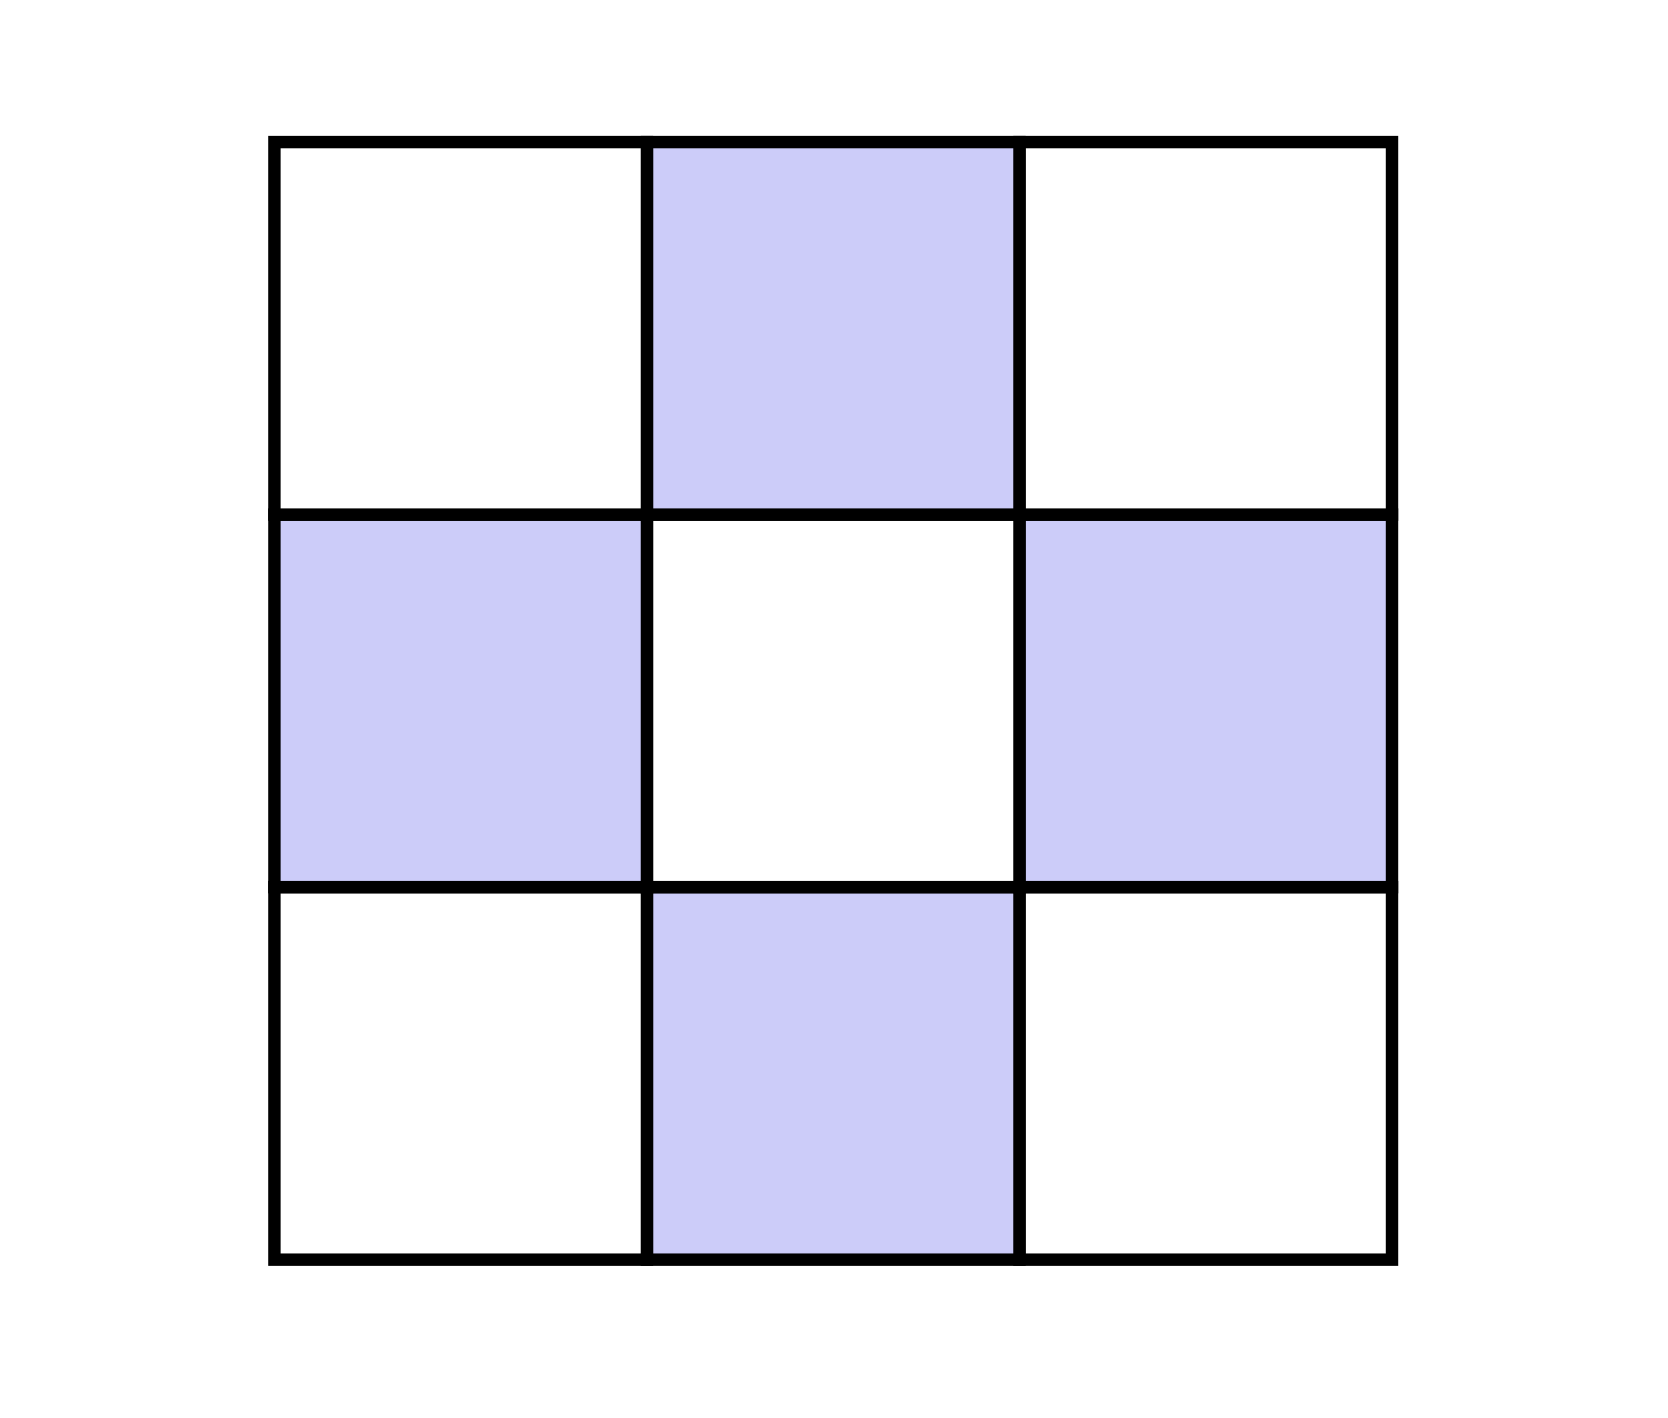
\includegraphics{class/imgdenoise/template-beta.png}

When we convolve this filter with an image, the result corresponds to
the majority pixel value in the patch over which we perform the
convolution. We can create an energy function using only the \(\beta\)
term to see the result of applying this median filter.

    \begin{Verbatim}[commandchars=\\\{\}]
{\color{incolor}In [{\color{incolor}10}]:} \PY{k}{def} \PY{n+nf}{defaultEnergyFunction}\PY{p}{(}\PY{n}{hidden}\PY{p}{,} \PY{n}{observation}\PY{p}{,} \PY{n}{alpha} \PY{o}{=} \PY{l+m+mi}{1}\PY{p}{,} \PY{n}{beta} \PY{o}{=} \PY{l+m+mi}{1}\PY{p}{,} \PY{n}{eta} \PY{o}{=} \PY{l+m+mi}{1}\PY{p}{)}\PY{p}{:}
             \PY{c+c1}{\PYZsh{} create filter for beta term}
             \PY{n}{Tb} \PY{o}{=} \PY{n}{np}\PY{o}{.}\PY{n}{asarray}\PY{p}{(}\PY{p}{[}\PY{p}{[}\PY{l+m+mi}{0}\PY{p}{,} \PY{l+m+mf}{1.0}\PY{p}{,} \PY{l+m+mi}{0}\PY{p}{]}\PY{p}{,} \PY{p}{[}\PY{l+m+mf}{1.0}\PY{p}{,} \PY{l+m+mi}{0}\PY{p}{,} \PY{l+m+mf}{1.0}\PY{p}{]}\PY{p}{,} \PY{p}{[}\PY{l+m+mi}{0}\PY{p}{,} \PY{l+m+mf}{1.0}\PY{p}{,} \PY{l+m+mi}{0}\PY{p}{]}\PY{p}{]}\PY{p}{)}
             \PY{c+c1}{\PYZsh{} convolve hidden image with term B\PYZsq{}s filter}
             \PY{n}{matB} \PY{o}{=} \PY{n}{conv2d}\PY{p}{(}\PY{n}{hidden}\PY{p}{,} \PY{n}{Tb}\PY{p}{,} \PY{l+s+s1}{\PYZsq{}}\PY{l+s+s1}{same}\PY{l+s+s1}{\PYZsq{}}\PY{p}{)}
             \PY{c+c1}{\PYZsh{} calculate energy map}
             \PY{n}{mapE} \PY{o}{=} \PY{n}{hidden} \PY{o}{*} \PY{p}{(}\PY{n}{alpha} \PY{o}{\PYZhy{}} \PY{n}{beta} \PY{o}{*} \PY{n}{matB} \PY{o}{\PYZhy{}} \PY{n}{eta} \PY{o}{*} \PY{n}{observation}\PY{p}{)}
             \PY{c+c1}{\PYZsh{} get mean of matrix as energy}
             \PY{n}{E} \PY{o}{=} \PY{n}{np}\PY{o}{.}\PY{n}{mean}\PY{p}{(}\PY{n}{mapE}\PY{p}{)}
             \PY{c+c1}{\PYZsh{} calculate energy difference map}
             \PY{n}{dE} \PY{o}{=} \PY{o}{\PYZhy{}}\PY{l+m+mi}{2} \PY{o}{*} \PY{n}{mapE}
             
             \PY{k}{return} \PY{n}{E}\PY{p}{,} \PY{n}{dE}
\end{Verbatim}


    \begin{Verbatim}[commandchars=\\\{\}]
{\color{incolor}In [{\color{incolor}11}]:} \PY{n}{medFilter} \PY{o}{=} \PY{k}{lambda} \PY{n}{hidden}\PY{p}{,} \PY{n}{observation}\PY{p}{:} \PY{n}{defaultEnergyFunction}\PY{p}{(}\PY{n}{hidden}\PY{p}{,} \PY{n}{observation}\PY{p}{,}
                                                                       \PY{n}{alpha}\PY{o}{=}\PY{l+m+mi}{0}\PY{p}{,} \PY{n}{beta}\PY{o}{=}\PY{l+m+mi}{1}\PY{p}{,} \PY{n}{eta}\PY{o}{=}\PY{l+m+mi}{0}\PY{p}{)}
\end{Verbatim}


    \begin{Verbatim}[commandchars=\\\{\}]
{\color{incolor}In [{\color{incolor}12}]:} \PY{n}{imrecMed} \PY{o}{=} \PY{n}{denoise}\PY{p}{(}\PY{n}{im\PYZus{}noisy}\PY{p}{,} \PY{n}{medFilter}\PY{p}{)}
         \PY{n}{showimgs}\PY{p}{(}\PY{n}{img}\PY{p}{,} \PY{n}{im\PYZus{}noisy}\PY{p}{,} \PY{n}{imrec}\PY{p}{,} \PY{n}{imrecMed}\PY{p}{)}
\end{Verbatim}


    \begin{center}
    \adjustimage{max size={0.9\linewidth}{0.9\paperheight}}{output_19_0.png}
    \end{center}
    { \hspace*{\fill} \\}
    
    As can be seen, the median filter by itself does a decent job of
decreasing the noise in the image, simply by taking the majority pixel
vlaue in each patch of the image. For this implementation, we are
assuming only that there is a relationship between neighboring pixels in
the hidden image.

    \hypertarget{improvement-of-default-energy-function}{%
\section{Improvement of Default Energy
Function}\label{improvement-of-default-energy-function}}

To improve the energy function, we can use different filter templates
for \(\beta\).

Several different templates are shown below:

\begin{longtable}[]{@{}ll@{}}
\toprule
\(T_{\alpha}\) & \(T_{\gamma}\)\tabularnewline
\midrule
\endhead
&\tabularnewline
\bottomrule
\end{longtable}

\begin{longtable}[]{@{}ll@{}}
\toprule
\(T_{\phi}\) & \(T_{\sigma}\)\tabularnewline
\midrule
\endhead
&\tabularnewline
\bottomrule
\end{longtable}

These templates are all 5 x 5 because a 3 x 3 filter cannot remove noise
that extends across more than two pixels. The new filters can be
implemented in the same way as the original filter by defining the
energy function with the filter convolved with the hidden image.

    \begin{Verbatim}[commandchars=\\\{\}]
{\color{incolor}In [{\color{incolor}13}]:} \PY{k}{def} \PY{n+nf}{extendEnergyFunction}\PY{p}{(}\PY{n}{hidden}\PY{p}{,} \PY{n}{observation}\PY{p}{,} 
                                  \PY{n}{alpha}\PY{o}{=}\PY{l+m+mi}{1}\PY{p}{,} \PY{n}{beta}\PY{o}{=}\PY{l+m+mi}{1}\PY{p}{,} \PY{n}{gamma}\PY{o}{=}\PY{l+m+mi}{1}\PY{p}{,} \PY{n}{phi}\PY{o}{=}\PY{l+m+mi}{1}\PY{p}{,} \PY{n}{sigma}\PY{o}{=}\PY{l+m+mi}{1}\PY{p}{,} \PY{n}{eta}\PY{o}{=}\PY{l+m+mi}{1}\PY{p}{)}\PY{p}{:}
             \PY{c+c1}{\PYZsh{} template alpha}
             \PY{n}{Ta} \PY{o}{=} \PY{n}{np}\PY{o}{.}\PY{n}{asarray}\PY{p}{(}\PY{p}{[}\PY{p}{[}\PY{p}{[}\PY{o}{\PYZhy{}}\PY{l+m+mi}{1}\PY{p}{,}\PY{o}{\PYZhy{}}\PY{l+m+mi}{1}\PY{p}{,}\PY{o}{\PYZhy{}}\PY{l+m+mi}{1}\PY{p}{,}\PY{o}{\PYZhy{}}\PY{l+m+mi}{1}\PY{p}{,}\PY{l+m+mi}{1}\PY{p}{]}\PY{p}{,}\PY{p}{[}\PY{o}{\PYZhy{}}\PY{l+m+mi}{1}\PY{p}{,}\PY{o}{\PYZhy{}}\PY{l+m+mi}{1}\PY{p}{,}\PY{o}{\PYZhy{}}\PY{l+m+mi}{1}\PY{p}{,}\PY{l+m+mi}{1}\PY{p}{,}\PY{o}{\PYZhy{}}\PY{l+m+mi}{1}\PY{p}{]}\PY{p}{,}\PY{p}{[}\PY{o}{\PYZhy{}}\PY{l+m+mi}{1}\PY{p}{,}\PY{o}{\PYZhy{}}\PY{l+m+mi}{1}\PY{p}{,}\PY{l+m+mi}{0}\PY{p}{,}\PY{o}{\PYZhy{}}\PY{l+m+mi}{1}\PY{p}{,}\PY{o}{\PYZhy{}}\PY{l+m+mi}{1}\PY{p}{]}\PY{p}{,}\PY{p}{[}\PY{o}{\PYZhy{}}\PY{l+m+mi}{1}\PY{p}{,}\PY{l+m+mi}{1}\PY{p}{,}\PY{o}{\PYZhy{}}\PY{l+m+mi}{1}\PY{p}{,}\PY{o}{\PYZhy{}}\PY{l+m+mi}{1}\PY{p}{,}\PY{o}{\PYZhy{}}\PY{l+m+mi}{1}\PY{p}{]}\PY{p}{,}\PY{p}{[}\PY{l+m+mi}{1}\PY{p}{,}\PY{o}{\PYZhy{}}\PY{l+m+mi}{1}\PY{p}{,}\PY{o}{\PYZhy{}}\PY{l+m+mi}{1}\PY{p}{,}\PY{o}{\PYZhy{}}\PY{l+m+mi}{1}\PY{p}{,}\PY{o}{\PYZhy{}}\PY{l+m+mi}{1}\PY{p}{]}\PY{p}{]}\PY{p}{,}
                              \PY{p}{[}\PY{p}{[}\PY{o}{\PYZhy{}}\PY{l+m+mi}{1}\PY{p}{,}\PY{o}{\PYZhy{}}\PY{l+m+mi}{1}\PY{p}{,}\PY{l+m+mi}{1}\PY{p}{,}\PY{o}{\PYZhy{}}\PY{l+m+mi}{1}\PY{p}{,}\PY{o}{\PYZhy{}}\PY{l+m+mi}{1}\PY{p}{]}\PY{p}{,}\PY{p}{[}\PY{o}{\PYZhy{}}\PY{l+m+mi}{1}\PY{p}{,}\PY{o}{\PYZhy{}}\PY{l+m+mi}{1}\PY{p}{,}\PY{l+m+mi}{1}\PY{p}{,}\PY{o}{\PYZhy{}}\PY{l+m+mi}{1}\PY{p}{,}\PY{o}{\PYZhy{}}\PY{l+m+mi}{1}\PY{p}{]}\PY{p}{,}\PY{p}{[}\PY{o}{\PYZhy{}}\PY{l+m+mi}{1}\PY{p}{,}\PY{o}{\PYZhy{}}\PY{l+m+mi}{1}\PY{p}{,}\PY{l+m+mi}{0}\PY{p}{,}\PY{o}{\PYZhy{}}\PY{l+m+mi}{1}\PY{p}{,}\PY{o}{\PYZhy{}}\PY{l+m+mi}{1}\PY{p}{]}\PY{p}{,}\PY{p}{[}\PY{o}{\PYZhy{}}\PY{l+m+mi}{1}\PY{p}{,}\PY{o}{\PYZhy{}}\PY{l+m+mi}{1}\PY{p}{,}\PY{l+m+mi}{1}\PY{p}{,}\PY{o}{\PYZhy{}}\PY{l+m+mi}{1}\PY{p}{,}\PY{o}{\PYZhy{}}\PY{l+m+mi}{1}\PY{p}{]}\PY{p}{,}\PY{p}{[}\PY{o}{\PYZhy{}}\PY{l+m+mi}{1}\PY{p}{,}\PY{o}{\PYZhy{}}\PY{l+m+mi}{1}\PY{p}{,}\PY{l+m+mi}{1}\PY{p}{,}\PY{o}{\PYZhy{}}\PY{l+m+mi}{1}\PY{p}{,}\PY{o}{\PYZhy{}}\PY{l+m+mi}{1}\PY{p}{]}\PY{p}{]}\PY{p}{,}
                              \PY{p}{[}\PY{p}{[}\PY{l+m+mi}{1}\PY{p}{,}\PY{o}{\PYZhy{}}\PY{l+m+mi}{1}\PY{p}{,}\PY{o}{\PYZhy{}}\PY{l+m+mi}{1}\PY{p}{,}\PY{o}{\PYZhy{}}\PY{l+m+mi}{1}\PY{p}{,}\PY{o}{\PYZhy{}}\PY{l+m+mi}{1}\PY{p}{]}\PY{p}{,}\PY{p}{[}\PY{o}{\PYZhy{}}\PY{l+m+mi}{1}\PY{p}{,}\PY{l+m+mi}{1}\PY{p}{,}\PY{o}{\PYZhy{}}\PY{l+m+mi}{1}\PY{p}{,}\PY{o}{\PYZhy{}}\PY{l+m+mi}{1}\PY{p}{,}\PY{o}{\PYZhy{}}\PY{l+m+mi}{1}\PY{p}{]}\PY{p}{,}\PY{p}{[}\PY{o}{\PYZhy{}}\PY{l+m+mi}{1}\PY{p}{,}\PY{o}{\PYZhy{}}\PY{l+m+mi}{1}\PY{p}{,}\PY{l+m+mi}{0}\PY{p}{,}\PY{o}{\PYZhy{}}\PY{l+m+mi}{1}\PY{p}{,}\PY{o}{\PYZhy{}}\PY{l+m+mi}{1}\PY{p}{]}\PY{p}{,}\PY{p}{[}\PY{o}{\PYZhy{}}\PY{l+m+mi}{1}\PY{p}{,}\PY{o}{\PYZhy{}}\PY{l+m+mi}{1}\PY{p}{,}\PY{o}{\PYZhy{}}\PY{l+m+mi}{1}\PY{p}{,}\PY{l+m+mi}{1}\PY{p}{,}\PY{o}{\PYZhy{}}\PY{l+m+mi}{1}\PY{p}{]}\PY{p}{,}\PY{p}{[}\PY{o}{\PYZhy{}}\PY{l+m+mi}{1}\PY{p}{,}\PY{o}{\PYZhy{}}\PY{l+m+mi}{1}\PY{p}{,}\PY{o}{\PYZhy{}}\PY{l+m+mi}{1}\PY{p}{,}\PY{o}{\PYZhy{}}\PY{l+m+mi}{1}\PY{p}{,}\PY{l+m+mi}{1}\PY{p}{]}\PY{p}{]}\PY{p}{,}
                              \PY{p}{[}\PY{p}{[}\PY{o}{\PYZhy{}}\PY{l+m+mi}{1}\PY{p}{,}\PY{o}{\PYZhy{}}\PY{l+m+mi}{1}\PY{p}{,}\PY{o}{\PYZhy{}}\PY{l+m+mi}{1}\PY{p}{,}\PY{o}{\PYZhy{}}\PY{l+m+mi}{1}\PY{p}{,}\PY{o}{\PYZhy{}}\PY{l+m+mi}{1}\PY{p}{]}\PY{p}{,}\PY{p}{[}\PY{o}{\PYZhy{}}\PY{l+m+mi}{1}\PY{p}{,}\PY{o}{\PYZhy{}}\PY{l+m+mi}{1}\PY{p}{,}\PY{o}{\PYZhy{}}\PY{l+m+mi}{1}\PY{p}{,}\PY{o}{\PYZhy{}}\PY{l+m+mi}{1}\PY{p}{,}\PY{o}{\PYZhy{}}\PY{l+m+mi}{1}\PY{p}{]}\PY{p}{,}\PY{p}{[}\PY{l+m+mi}{1}\PY{p}{,}\PY{l+m+mi}{1}\PY{p}{,}\PY{l+m+mi}{0}\PY{p}{,}\PY{l+m+mi}{1}\PY{p}{,}\PY{l+m+mi}{1}\PY{p}{]}\PY{p}{,}\PY{p}{[}\PY{o}{\PYZhy{}}\PY{l+m+mi}{1}\PY{p}{,}\PY{o}{\PYZhy{}}\PY{l+m+mi}{1}\PY{p}{,}\PY{o}{\PYZhy{}}\PY{l+m+mi}{1}\PY{p}{,}\PY{o}{\PYZhy{}}\PY{l+m+mi}{1}\PY{p}{,}\PY{o}{\PYZhy{}}\PY{l+m+mi}{1}\PY{p}{]}\PY{p}{,}\PY{p}{[}\PY{o}{\PYZhy{}}\PY{l+m+mi}{1}\PY{p}{,}\PY{o}{\PYZhy{}}\PY{l+m+mi}{1}\PY{p}{,}\PY{o}{\PYZhy{}}\PY{l+m+mi}{1}\PY{p}{,}\PY{o}{\PYZhy{}}\PY{l+m+mi}{1}\PY{p}{,}\PY{o}{\PYZhy{}}\PY{l+m+mi}{1}\PY{p}{]}\PY{p}{]}\PY{p}{]}\PY{p}{)}
             \PY{c+c1}{\PYZsh{} template beta}
             \PY{n}{Tb} \PY{o}{=} \PY{n}{np}\PY{o}{.}\PY{n}{asarray}\PY{p}{(}\PY{p}{[}\PY{p}{[}\PY{l+m+mi}{0}\PY{p}{,} \PY{l+m+mi}{1}\PY{p}{,} \PY{l+m+mi}{0}\PY{p}{]}\PY{p}{,} \PY{p}{[}\PY{l+m+mi}{1}\PY{p}{,} \PY{l+m+mi}{0}\PY{p}{,} \PY{l+m+mi}{1}\PY{p}{]}\PY{p}{,} \PY{p}{[}\PY{l+m+mi}{0}\PY{p}{,} \PY{l+m+mi}{1}\PY{p}{,} \PY{l+m+mi}{0}\PY{p}{]}\PY{p}{]}\PY{p}{)}
             \PY{c+c1}{\PYZsh{} template gamma}
             \PY{n}{Tr} \PY{o}{=} \PY{n}{np}\PY{o}{.}\PY{n}{asarray}\PY{p}{(}\PY{p}{[}\PY{p}{[}\PY{l+m+mi}{1}\PY{p}{,}\PY{l+m+mi}{1}\PY{p}{,}\PY{l+m+mi}{1}\PY{p}{,}\PY{l+m+mi}{1}\PY{p}{,}\PY{l+m+mi}{1}\PY{p}{]}\PY{p}{,}\PY{p}{[}\PY{l+m+mi}{1}\PY{p}{,}\PY{l+m+mi}{0}\PY{p}{,}\PY{l+m+mi}{0}\PY{p}{,}\PY{l+m+mi}{0}\PY{p}{,}\PY{l+m+mi}{1}\PY{p}{]}\PY{p}{,}\PY{p}{[}\PY{l+m+mi}{1}\PY{p}{,}\PY{l+m+mi}{0}\PY{p}{,}\PY{l+m+mi}{0}\PY{p}{,}\PY{l+m+mi}{0}\PY{p}{,}\PY{l+m+mi}{1}\PY{p}{]}\PY{p}{,}\PY{p}{[}\PY{l+m+mi}{1}\PY{p}{,}\PY{l+m+mi}{0}\PY{p}{,}\PY{l+m+mi}{0}\PY{p}{,}\PY{l+m+mi}{0}\PY{p}{,}\PY{l+m+mi}{1}\PY{p}{]}\PY{p}{,}\PY{p}{[}\PY{l+m+mi}{1}\PY{p}{,}\PY{l+m+mi}{1}\PY{p}{,}\PY{l+m+mi}{1}\PY{p}{,}\PY{l+m+mi}{1}\PY{p}{,}\PY{l+m+mi}{1}\PY{p}{]}\PY{p}{]}\PY{p}{)}
             \PY{c+c1}{\PYZsh{} template phi}
             \PY{n}{Tp} \PY{o}{=} \PY{n}{np}\PY{o}{.}\PY{n}{asarray}\PY{p}{(}\PY{p}{[}\PY{p}{[}\PY{l+m+mi}{0}\PY{p}{,}\PY{l+m+mi}{0}\PY{p}{,}\PY{l+m+mi}{1}\PY{p}{,}\PY{l+m+mi}{0}\PY{p}{,}\PY{l+m+mi}{0}\PY{p}{]}\PY{p}{,}\PY{p}{[}\PY{l+m+mi}{0}\PY{p}{,}\PY{l+m+mi}{0}\PY{p}{,}\PY{l+m+mi}{1}\PY{p}{,}\PY{l+m+mi}{0}\PY{p}{,}\PY{l+m+mi}{0}\PY{p}{]}\PY{p}{,}\PY{p}{[}\PY{l+m+mi}{1}\PY{p}{,}\PY{l+m+mi}{1}\PY{p}{,}\PY{l+m+mi}{0}\PY{p}{,}\PY{l+m+mi}{1}\PY{p}{,}\PY{l+m+mi}{1}\PY{p}{]}\PY{p}{,}\PY{p}{[}\PY{l+m+mi}{0}\PY{p}{,}\PY{l+m+mi}{0}\PY{p}{,}\PY{l+m+mi}{1}\PY{p}{,}\PY{l+m+mi}{0}\PY{p}{,}\PY{l+m+mi}{0}\PY{p}{]}\PY{p}{,}\PY{p}{[}\PY{l+m+mi}{0}\PY{p}{,}\PY{l+m+mi}{0}\PY{p}{,}\PY{l+m+mi}{1}\PY{p}{,}\PY{l+m+mi}{0}\PY{p}{,}\PY{l+m+mi}{0}\PY{p}{]}\PY{p}{]}\PY{p}{)}
             \PY{c+c1}{\PYZsh{} template sigma}
             \PY{n}{Ts} \PY{o}{=} \PY{n}{np}\PY{o}{.}\PY{n}{asarray}\PY{p}{(}\PY{p}{[}\PY{p}{[}\PY{p}{[}\PY{l+m+mi}{1}\PY{p}{,}\PY{o}{\PYZhy{}}\PY{l+m+mi}{1}\PY{p}{,}\PY{o}{\PYZhy{}}\PY{l+m+mi}{1}\PY{p}{,}\PY{o}{\PYZhy{}}\PY{l+m+mi}{1}\PY{p}{,}\PY{o}{\PYZhy{}}\PY{l+m+mi}{1}\PY{p}{]}\PY{p}{,}\PY{p}{[}\PY{l+m+mi}{1}\PY{p}{,}\PY{l+m+mi}{0}\PY{p}{,}\PY{o}{\PYZhy{}}\PY{l+m+mi}{1}\PY{p}{,}\PY{o}{\PYZhy{}}\PY{l+m+mi}{1}\PY{p}{,}\PY{o}{\PYZhy{}}\PY{l+m+mi}{1}\PY{p}{]}\PY{p}{,}\PY{p}{[}\PY{l+m+mi}{1}\PY{p}{,}\PY{l+m+mi}{1}\PY{p}{,}\PY{l+m+mi}{0}\PY{p}{,}\PY{o}{\PYZhy{}}\PY{l+m+mi}{1}\PY{p}{,}\PY{o}{\PYZhy{}}\PY{l+m+mi}{1}\PY{p}{]}\PY{p}{,}\PY{p}{[}\PY{l+m+mi}{1}\PY{p}{,}\PY{l+m+mi}{1}\PY{p}{,}\PY{l+m+mi}{1}\PY{p}{,}\PY{l+m+mi}{0}\PY{p}{,}\PY{o}{\PYZhy{}}\PY{l+m+mi}{1}\PY{p}{]}\PY{p}{,}\PY{p}{[}\PY{l+m+mi}{1}\PY{p}{,}\PY{l+m+mi}{1}\PY{p}{,}\PY{l+m+mi}{1}\PY{p}{,}\PY{l+m+mi}{1}\PY{p}{,}\PY{l+m+mi}{1}\PY{p}{]}\PY{p}{]}\PY{p}{,}
                              \PY{p}{[}\PY{p}{[}\PY{l+m+mi}{1}\PY{p}{,}\PY{l+m+mi}{1}\PY{p}{,}\PY{l+m+mi}{1}\PY{p}{,}\PY{o}{\PYZhy{}}\PY{l+m+mi}{1}\PY{p}{,}\PY{o}{\PYZhy{}}\PY{l+m+mi}{1}\PY{p}{]}\PY{p}{,}\PY{p}{[}\PY{l+m+mi}{1}\PY{p}{,}\PY{l+m+mi}{1}\PY{p}{,}\PY{l+m+mi}{0}\PY{p}{,}\PY{o}{\PYZhy{}}\PY{l+m+mi}{1}\PY{p}{,}\PY{o}{\PYZhy{}}\PY{l+m+mi}{1}\PY{p}{]}\PY{p}{,}\PY{p}{[}\PY{l+m+mi}{1}\PY{p}{,}\PY{l+m+mi}{1}\PY{p}{,}\PY{l+m+mi}{0}\PY{p}{,}\PY{o}{\PYZhy{}}\PY{l+m+mi}{1}\PY{p}{,}\PY{o}{\PYZhy{}}\PY{l+m+mi}{1}\PY{p}{]}\PY{p}{,}\PY{p}{[}\PY{l+m+mi}{1}\PY{p}{,}\PY{l+m+mi}{1}\PY{p}{,}\PY{l+m+mi}{0}\PY{p}{,}\PY{o}{\PYZhy{}}\PY{l+m+mi}{1}\PY{p}{,}\PY{o}{\PYZhy{}}\PY{l+m+mi}{1}\PY{p}{]}\PY{p}{,}\PY{p}{[}\PY{l+m+mi}{1}\PY{p}{,}\PY{l+m+mi}{1}\PY{p}{,}\PY{l+m+mi}{1}\PY{p}{,}\PY{o}{\PYZhy{}}\PY{l+m+mi}{1}\PY{p}{,}\PY{o}{\PYZhy{}}\PY{l+m+mi}{1}\PY{p}{]}\PY{p}{]}\PY{p}{,}
                              \PY{p}{[}\PY{p}{[}\PY{l+m+mi}{1}\PY{p}{,}\PY{l+m+mi}{1}\PY{p}{,}\PY{l+m+mi}{1}\PY{p}{,}\PY{l+m+mi}{1}\PY{p}{,}\PY{l+m+mi}{1}\PY{p}{]}\PY{p}{,}\PY{p}{[}\PY{l+m+mi}{1}\PY{p}{,}\PY{l+m+mi}{1}\PY{p}{,}\PY{l+m+mi}{1}\PY{p}{,}\PY{l+m+mi}{0}\PY{p}{,}\PY{o}{\PYZhy{}}\PY{l+m+mi}{1}\PY{p}{]}\PY{p}{,}\PY{p}{[}\PY{l+m+mi}{1}\PY{p}{,}\PY{l+m+mi}{1}\PY{p}{,}\PY{l+m+mi}{0}\PY{p}{,}\PY{o}{\PYZhy{}}\PY{l+m+mi}{1}\PY{p}{,}\PY{o}{\PYZhy{}}\PY{l+m+mi}{1}\PY{p}{]}\PY{p}{,}\PY{p}{[}\PY{l+m+mi}{1}\PY{p}{,}\PY{l+m+mi}{0}\PY{p}{,}\PY{o}{\PYZhy{}}\PY{l+m+mi}{1}\PY{p}{,}\PY{o}{\PYZhy{}}\PY{l+m+mi}{1}\PY{p}{,}\PY{o}{\PYZhy{}}\PY{l+m+mi}{1}\PY{p}{]}\PY{p}{,}\PY{p}{[}\PY{l+m+mi}{1}\PY{p}{,}\PY{o}{\PYZhy{}}\PY{l+m+mi}{1}\PY{p}{,}\PY{o}{\PYZhy{}}\PY{l+m+mi}{1}\PY{p}{,}\PY{o}{\PYZhy{}}\PY{l+m+mi}{1}\PY{p}{,}\PY{o}{\PYZhy{}}\PY{l+m+mi}{1}\PY{p}{]}\PY{p}{]}\PY{p}{,}
                              \PY{p}{[}\PY{p}{[}\PY{l+m+mi}{1}\PY{p}{,}\PY{l+m+mi}{1}\PY{p}{,}\PY{l+m+mi}{1}\PY{p}{,}\PY{l+m+mi}{1}\PY{p}{,}\PY{l+m+mi}{1}\PY{p}{]}\PY{p}{,}\PY{p}{[}\PY{l+m+mi}{1}\PY{p}{,}\PY{l+m+mi}{1}\PY{p}{,}\PY{l+m+mi}{1}\PY{p}{,}\PY{l+m+mi}{1}\PY{p}{,}\PY{l+m+mi}{1}\PY{p}{]}\PY{p}{,}\PY{p}{[}\PY{l+m+mi}{1}\PY{p}{,}\PY{l+m+mi}{0}\PY{p}{,}\PY{l+m+mi}{0}\PY{p}{,}\PY{l+m+mi}{0}\PY{p}{,}\PY{l+m+mi}{1}\PY{p}{]}\PY{p}{,}\PY{p}{[}\PY{o}{\PYZhy{}}\PY{l+m+mi}{1}\PY{p}{,}\PY{o}{\PYZhy{}}\PY{l+m+mi}{1}\PY{p}{,}\PY{o}{\PYZhy{}}\PY{l+m+mi}{1}\PY{p}{,}\PY{o}{\PYZhy{}}\PY{l+m+mi}{1}\PY{p}{,}\PY{o}{\PYZhy{}}\PY{l+m+mi}{1}\PY{p}{]}\PY{p}{,}\PY{p}{[}\PY{o}{\PYZhy{}}\PY{l+m+mi}{1}\PY{p}{,}\PY{o}{\PYZhy{}}\PY{l+m+mi}{1}\PY{p}{,}\PY{o}{\PYZhy{}}\PY{l+m+mi}{1}\PY{p}{,}\PY{o}{\PYZhy{}}\PY{l+m+mi}{1}\PY{p}{,}\PY{o}{\PYZhy{}}\PY{l+m+mi}{1}\PY{p}{]}\PY{p}{]}\PY{p}{,}
                              \PY{p}{[}\PY{p}{[}\PY{l+m+mi}{1}\PY{p}{,}\PY{l+m+mi}{1}\PY{p}{,}\PY{l+m+mi}{1}\PY{p}{,}\PY{l+m+mi}{1}\PY{p}{,}\PY{l+m+mi}{1}\PY{p}{]}\PY{p}{,}\PY{p}{[}\PY{o}{\PYZhy{}}\PY{l+m+mi}{1}\PY{p}{,}\PY{l+m+mi}{0}\PY{p}{,}\PY{l+m+mi}{1}\PY{p}{,}\PY{l+m+mi}{1}\PY{p}{,}\PY{l+m+mi}{1}\PY{p}{]}\PY{p}{,}\PY{p}{[}\PY{o}{\PYZhy{}}\PY{l+m+mi}{1}\PY{p}{,}\PY{o}{\PYZhy{}}\PY{l+m+mi}{1}\PY{p}{,}\PY{l+m+mi}{0}\PY{p}{,}\PY{l+m+mi}{1}\PY{p}{,}\PY{l+m+mi}{1}\PY{p}{]}\PY{p}{,}\PY{p}{[}\PY{o}{\PYZhy{}}\PY{l+m+mi}{1}\PY{p}{,}\PY{o}{\PYZhy{}}\PY{l+m+mi}{1}\PY{p}{,}\PY{o}{\PYZhy{}}\PY{l+m+mi}{1}\PY{p}{,}\PY{l+m+mi}{0}\PY{p}{,}\PY{l+m+mi}{1}\PY{p}{]}\PY{p}{,}\PY{p}{[}\PY{o}{\PYZhy{}}\PY{l+m+mi}{1}\PY{p}{,}\PY{o}{\PYZhy{}}\PY{l+m+mi}{1}\PY{p}{,}\PY{o}{\PYZhy{}}\PY{l+m+mi}{1}\PY{p}{,}\PY{o}{\PYZhy{}}\PY{l+m+mi}{1}\PY{p}{,}\PY{l+m+mi}{1}\PY{p}{]}\PY{p}{]}\PY{p}{,}
                              \PY{p}{[}\PY{p}{[}\PY{o}{\PYZhy{}}\PY{l+m+mi}{1}\PY{p}{,}\PY{o}{\PYZhy{}}\PY{l+m+mi}{1}\PY{p}{,}\PY{l+m+mi}{1}\PY{p}{,}\PY{l+m+mi}{1}\PY{p}{,}\PY{l+m+mi}{1}\PY{p}{]}\PY{p}{,}\PY{p}{[}\PY{o}{\PYZhy{}}\PY{l+m+mi}{1}\PY{p}{,}\PY{o}{\PYZhy{}}\PY{l+m+mi}{1}\PY{p}{,}\PY{l+m+mi}{0}\PY{p}{,}\PY{l+m+mi}{1}\PY{p}{,}\PY{l+m+mi}{1}\PY{p}{]}\PY{p}{,}\PY{p}{[}\PY{o}{\PYZhy{}}\PY{l+m+mi}{1}\PY{p}{,}\PY{o}{\PYZhy{}}\PY{l+m+mi}{1}\PY{p}{,}\PY{l+m+mi}{0}\PY{p}{,}\PY{l+m+mi}{1}\PY{p}{,}\PY{l+m+mi}{1}\PY{p}{]}\PY{p}{,}\PY{p}{[}\PY{o}{\PYZhy{}}\PY{l+m+mi}{1}\PY{p}{,}\PY{o}{\PYZhy{}}\PY{l+m+mi}{1}\PY{p}{,}\PY{l+m+mi}{0}\PY{p}{,}\PY{l+m+mi}{1}\PY{p}{,}\PY{l+m+mi}{1}\PY{p}{]}\PY{p}{,}\PY{p}{[}\PY{o}{\PYZhy{}}\PY{l+m+mi}{1}\PY{p}{,}\PY{o}{\PYZhy{}}\PY{l+m+mi}{1}\PY{p}{,}\PY{l+m+mi}{1}\PY{p}{,}\PY{l+m+mi}{1}\PY{p}{,}\PY{l+m+mi}{1}\PY{p}{]}\PY{p}{]}\PY{p}{,}
                              \PY{p}{[}\PY{p}{[}\PY{o}{\PYZhy{}}\PY{l+m+mi}{1}\PY{p}{,}\PY{o}{\PYZhy{}}\PY{l+m+mi}{1}\PY{p}{,}\PY{o}{\PYZhy{}}\PY{l+m+mi}{1}\PY{p}{,}\PY{o}{\PYZhy{}}\PY{l+m+mi}{1}\PY{p}{,}\PY{l+m+mi}{1}\PY{p}{]}\PY{p}{,}\PY{p}{[}\PY{o}{\PYZhy{}}\PY{l+m+mi}{1}\PY{p}{,}\PY{o}{\PYZhy{}}\PY{l+m+mi}{1}\PY{p}{,}\PY{o}{\PYZhy{}}\PY{l+m+mi}{1}\PY{p}{,}\PY{l+m+mi}{0}\PY{p}{,}\PY{l+m+mi}{1}\PY{p}{]}\PY{p}{,}\PY{p}{[}\PY{o}{\PYZhy{}}\PY{l+m+mi}{1}\PY{p}{,}\PY{o}{\PYZhy{}}\PY{l+m+mi}{1}\PY{p}{,}\PY{l+m+mi}{0}\PY{p}{,}\PY{l+m+mi}{1}\PY{p}{,}\PY{l+m+mi}{1}\PY{p}{]}\PY{p}{,}\PY{p}{[}\PY{o}{\PYZhy{}}\PY{l+m+mi}{1}\PY{p}{,}\PY{l+m+mi}{0}\PY{p}{,}\PY{l+m+mi}{1}\PY{p}{,}\PY{l+m+mi}{1}\PY{p}{,}\PY{l+m+mi}{1}\PY{p}{]}\PY{p}{,}\PY{p}{[}\PY{l+m+mi}{1}\PY{p}{,}\PY{l+m+mi}{1}\PY{p}{,}\PY{l+m+mi}{1}\PY{p}{,}\PY{l+m+mi}{1}\PY{p}{,}\PY{l+m+mi}{1}\PY{p}{]}\PY{p}{]}\PY{p}{,}
                              \PY{p}{[}\PY{p}{[}\PY{o}{\PYZhy{}}\PY{l+m+mi}{1}\PY{p}{,}\PY{o}{\PYZhy{}}\PY{l+m+mi}{1}\PY{p}{,}\PY{o}{\PYZhy{}}\PY{l+m+mi}{1}\PY{p}{,}\PY{o}{\PYZhy{}}\PY{l+m+mi}{1}\PY{p}{,}\PY{o}{\PYZhy{}}\PY{l+m+mi}{1}\PY{p}{]}\PY{p}{,}\PY{p}{[}\PY{o}{\PYZhy{}}\PY{l+m+mi}{1}\PY{p}{,}\PY{o}{\PYZhy{}}\PY{l+m+mi}{1}\PY{p}{,}\PY{o}{\PYZhy{}}\PY{l+m+mi}{1}\PY{p}{,}\PY{o}{\PYZhy{}}\PY{l+m+mi}{1}\PY{p}{,}\PY{o}{\PYZhy{}}\PY{l+m+mi}{1}\PY{p}{]}\PY{p}{,}\PY{p}{[}\PY{l+m+mi}{1}\PY{p}{,}\PY{l+m+mi}{0}\PY{p}{,}\PY{l+m+mi}{0}\PY{p}{,}\PY{l+m+mi}{0}\PY{p}{,}\PY{l+m+mi}{1}\PY{p}{]}\PY{p}{,}\PY{p}{[}\PY{l+m+mi}{1}\PY{p}{,}\PY{l+m+mi}{1}\PY{p}{,}\PY{l+m+mi}{1}\PY{p}{,}\PY{l+m+mi}{1}\PY{p}{,}\PY{l+m+mi}{1}\PY{p}{]}\PY{p}{,}\PY{p}{[}\PY{l+m+mi}{1}\PY{p}{,}\PY{l+m+mi}{1}\PY{p}{,}\PY{l+m+mi}{1}\PY{p}{,}\PY{l+m+mi}{1}\PY{p}{,}\PY{l+m+mi}{1}\PY{p}{]}\PY{p}{]}\PY{p}{]}\PY{p}{)}
             
             \PY{c+c1}{\PYZsh{} generate parameter matrix alpha}
             \PY{n}{matA} \PY{o}{=} \PY{n}{np}\PY{o}{.}\PY{n}{empty}\PY{p}{(}\PY{n}{hidden}\PY{o}{.}\PY{n}{shape}\PY{p}{)}
             \PY{k}{for} \PY{n}{T} \PY{o+ow}{in} \PY{n}{Ta}\PY{p}{:}
                 \PY{n}{matA} \PY{o}{=} \PY{n}{np}\PY{o}{.}\PY{n}{maximum}\PY{p}{(}\PY{n}{matA}\PY{p}{,} \PY{n}{hidden} \PY{o}{*} \PY{n}{conv2d}\PY{p}{(}\PY{n}{hidden}\PY{p}{,} \PY{n}{T}\PY{p}{,} \PY{l+s+s1}{\PYZsq{}}\PY{l+s+s1}{same}\PY{l+s+s1}{\PYZsq{}}\PY{p}{)}\PY{p}{)}
             \PY{c+c1}{\PYZsh{} generate parameter matrix beta}
             \PY{n}{matB} \PY{o}{=} \PY{n}{conv2d}\PY{p}{(}\PY{n}{hidden}\PY{p}{,} \PY{n}{Tb}\PY{p}{,} \PY{l+s+s1}{\PYZsq{}}\PY{l+s+s1}{same}\PY{l+s+s1}{\PYZsq{}}\PY{p}{)}
             \PY{c+c1}{\PYZsh{} generate parameter matrix gamma}
             \PY{n}{matR} \PY{o}{=} \PY{n}{conv2d}\PY{p}{(}\PY{n}{hidden}\PY{p}{,} \PY{n}{Tr}\PY{p}{,} \PY{l+s+s1}{\PYZsq{}}\PY{l+s+s1}{same}\PY{l+s+s1}{\PYZsq{}}\PY{p}{)}
             \PY{c+c1}{\PYZsh{} generate parameter matrix phi}
             \PY{n}{matP} \PY{o}{=} \PY{n}{conv2d}\PY{p}{(}\PY{n}{hidden}\PY{p}{,} \PY{n}{Tp}\PY{p}{,} \PY{l+s+s1}{\PYZsq{}}\PY{l+s+s1}{same}\PY{l+s+s1}{\PYZsq{}}\PY{p}{)}
             \PY{c+c1}{\PYZsh{} generate parameter matrix sigma}
             \PY{n}{matS} \PY{o}{=} \PY{n}{np}\PY{o}{.}\PY{n}{empty}\PY{p}{(}\PY{n}{hidden}\PY{o}{.}\PY{n}{shape}\PY{p}{)}
             \PY{k}{for} \PY{n}{T} \PY{o+ow}{in} \PY{n}{Ts}\PY{p}{:}
                 \PY{n}{matS} \PY{o}{=} \PY{n}{np}\PY{o}{.}\PY{n}{maximum}\PY{p}{(}\PY{n}{matS}\PY{p}{,} \PY{n}{hidden} \PY{o}{*} \PY{n}{conv2d}\PY{p}{(}\PY{n}{hidden}\PY{p}{,} \PY{n}{T}\PY{p}{,} \PY{l+s+s1}{\PYZsq{}}\PY{l+s+s1}{same}\PY{l+s+s1}{\PYZsq{}}\PY{p}{)}\PY{p}{)}
                 
             \PY{c+c1}{\PYZsh{} calculate energy map}
             \PY{n}{mapE} \PY{o}{=} \PY{o}{\PYZhy{}}\PY{n}{alpha}\PY{o}{*}\PY{n}{matA} \PY{o}{\PYZhy{}} \PY{n}{sigma}\PY{o}{*}\PY{n}{matS} \PY{o}{\PYZhy{}} \PY{n}{hidden}\PY{o}{*}\PY{p}{(}\PY{n}{beta}\PY{o}{*}\PY{n}{matB} \PY{o}{+} \PY{n}{gamma}\PY{o}{*}\PY{n}{matR} \PY{o}{+} \PY{n}{phi}\PY{o}{*}\PY{n}{matP} \PY{o}{+} \PY{n}{eta}\PY{o}{*}\PY{n}{observation}\PY{p}{)}
             \PY{c+c1}{\PYZsh{} get energy value as mean of map}
             \PY{n}{E} \PY{o}{=} \PY{n}{np}\PY{o}{.}\PY{n}{mean}\PY{p}{(}\PY{n}{mapE}\PY{p}{)}
             \PY{c+c1}{\PYZsh{} calculate energy difference map}
             \PY{n}{dE} \PY{o}{=} \PY{o}{\PYZhy{}}\PY{l+m+mi}{2} \PY{o}{*} \PY{n}{mapE}
             
             \PY{k}{return} \PY{n}{E}\PY{p}{,} \PY{n}{dE}
\end{Verbatim}


    \begin{Verbatim}[commandchars=\\\{\}]
{\color{incolor}In [{\color{incolor}14}]:} \PY{n}{medFilterExt} \PY{o}{=} \PY{k}{lambda} \PY{n}{hidden}\PY{p}{,} \PY{n}{observation}\PY{p}{:} \PY{n}{extendEnergyFunction}\PY{p}{(}\PY{n}{hidden}\PY{p}{,} \PY{n}{observation}\PY{p}{,} 
                                                                         \PY{n}{alpha}\PY{o}{=}\PY{l+m+mi}{0}\PY{p}{,} \PY{n}{beta}\PY{o}{=}\PY{l+m+mi}{1}\PY{p}{,} \PY{n}{gamma}\PY{o}{=}\PY{l+m+mf}{0.1}\PY{p}{,} 
                                                                         \PY{n}{phi}\PY{o}{=}\PY{l+m+mi}{0}\PY{p}{,} \PY{n}{sigma}\PY{o}{=}\PY{l+m+mi}{0}\PY{p}{,} \PY{n}{eta}\PY{o}{=}\PY{l+m+mi}{0}\PY{p}{)}
         
         \PY{n}{medFilterLarge} \PY{o}{=} \PY{k}{lambda} \PY{n}{hidden}\PY{p}{,} \PY{n}{observation}\PY{p}{:} \PY{n}{extendEnergyFunction}\PY{p}{(}\PY{n}{hidden}\PY{p}{,} \PY{n}{observation}\PY{p}{,} 
                                                                           \PY{n}{alpha}\PY{o}{=}\PY{l+m+mi}{0}\PY{p}{,} \PY{n}{beta}\PY{o}{=}\PY{l+m+mi}{0}\PY{p}{,} \PY{n}{gamma}\PY{o}{=}\PY{l+m+mi}{0}\PY{p}{,} 
                                                                           \PY{n}{phi}\PY{o}{=}\PY{l+m+mi}{1}\PY{p}{,} \PY{n}{sigma}\PY{o}{=}\PY{l+m+mi}{0}\PY{p}{,} \PY{n}{eta}\PY{o}{=}\PY{l+m+mi}{0}\PY{p}{)}
         
         \PY{c+c1}{\PYZsh{} denoise image with new energy functions}
         \PY{n}{imrecMedExt} \PY{o}{=} \PY{n}{denoise}\PY{p}{(}\PY{n}{im\PYZus{}noisy}\PY{p}{,} \PY{n}{medFilterExt}\PY{p}{)}
         \PY{n}{imrecMedLag} \PY{o}{=} \PY{n}{denoise}\PY{p}{(}\PY{n}{im\PYZus{}noisy}\PY{p}{,} \PY{n}{medFilterLarge}\PY{p}{)}
         
         \PY{c+c1}{\PYZsh{} compare result from different median filter}
         \PY{n}{showimgs}\PY{p}{(}\PY{n}{im\PYZus{}noisy}\PY{p}{,} \PY{n}{imrecMed}\PY{p}{,} \PY{n}{imrecMedExt}\PY{p}{,} \PY{n}{imrecMedLag}\PY{p}{)}
\end{Verbatim}


    \begin{center}
    \adjustimage{max size={0.9\linewidth}{0.9\paperheight}}{output_23_0.png}
    \end{center}
    { \hspace*{\fill} \\}
    
    \hypertarget{handling-edges}{%
\section{Handling Edges}\label{handling-edges}}

The final implementation in this notebook using filters that prevent
edge corrosion. These should speed up optimization, but will not further
improve the filtering results.

    \begin{Verbatim}[commandchars=\\\{\}]
{\color{incolor}In [{\color{incolor}15}]:} \PY{n}{medFilterProtectA} \PY{o}{=} \PY{k}{lambda} \PY{n}{hidden}\PY{p}{,} \PY{n}{observation}\PY{p}{:} \PY{n}{extendEnergyFunction}\PY{p}{(}\PY{n}{hidden}\PY{p}{,} \PY{n}{observation}\PY{p}{,} 
                                                                              \PY{n}{alpha}\PY{o}{=}\PY{l+m+mf}{0.1}\PY{p}{,} \PY{n}{beta}\PY{o}{=}\PY{l+m+mi}{1}\PY{p}{,} \PY{n}{gamma}\PY{o}{=}\PY{l+m+mf}{0.1}\PY{p}{,} 
                                                                              \PY{n}{phi}\PY{o}{=}\PY{l+m+mi}{0}\PY{p}{,} \PY{n}{sigma}\PY{o}{=}\PY{l+m+mi}{0}\PY{p}{,} \PY{n}{eta}\PY{o}{=}\PY{l+m+mi}{0}\PY{p}{)}
         
         \PY{n}{medFilterProtectS} \PY{o}{=} \PY{k}{lambda} \PY{n}{hidden}\PY{p}{,} \PY{n}{observation}\PY{p}{:} \PY{n}{extendEnergyFunction}\PY{p}{(}\PY{n}{hidden}\PY{p}{,} \PY{n}{observation}\PY{p}{,} 
                                                                              \PY{n}{alpha}\PY{o}{=}\PY{l+m+mi}{0}\PY{p}{,} \PY{n}{beta}\PY{o}{=}\PY{l+m+mi}{1}\PY{p}{,} \PY{n}{gamma}\PY{o}{=}\PY{l+m+mf}{0.1}\PY{p}{,} 
                                                                              \PY{n}{phi}\PY{o}{=}\PY{l+m+mi}{0}\PY{p}{,} \PY{n}{sigma}\PY{o}{=}\PY{l+m+mf}{0.1}\PY{p}{,} \PY{n}{eta}\PY{o}{=}\PY{l+m+mi}{0}\PY{p}{)}
         
         \PY{c+c1}{\PYZsh{} denoise image with new energy functions}
         \PY{n}{imrecMedProtectA} \PY{o}{=} \PY{n}{denoise}\PY{p}{(}\PY{n}{im\PYZus{}noisy}\PY{p}{,} \PY{n}{medFilterProtectA}\PY{p}{)}
         \PY{n}{imrecMedProtectS} \PY{o}{=} \PY{n}{denoise}\PY{p}{(}\PY{n}{im\PYZus{}noisy}\PY{p}{,} \PY{n}{medFilterProtectS}\PY{p}{)}
         
         \PY{c+c1}{\PYZsh{} compare result from different median filter}
         \PY{n}{showimgs}\PY{p}{(}\PY{n}{im\PYZus{}noisy}\PY{p}{,} \PY{n}{imrecMedExt}\PY{p}{,} \PY{n}{imrecMedProtectA}\PY{p}{,} \PY{n}{imrecMedProtectS}\PY{p}{)}
\end{Verbatim}


    \begin{center}
    \adjustimage{max size={0.9\linewidth}{0.9\paperheight}}{output_25_0.png}
    \end{center}
    { \hspace*{\fill} \\}
    
    \hypertarget{conclusions}{%
\section{Conclusions}\label{conclusions}}

In this notebook we saw how we could use a graphical model of an image
to remove random noise from an image. The model works by assuming that
cliques (adjacent pixels) in the hidden image should hve the same value,
and that corresponding pixels in the hidden and observed images should
have the same value. We also saw that we could add a term to bias the
results toward one particular pixel value. The process works by
calculating a loss (energy) as a function of the hidden and observed
image of the form:

\[E(X,Y) = \alpha\sum\limits_{i} x_i - \beta \sum\limits_{i,j} x_i x_j - \eta \sum\limits_{i} x_i y_i \]

The process to de-noise an image requires using gradient descent to find
the pixel values that minimize the energy function. Gradient descent is
an iterative approach that calculates the value of the loss function and
the gradient of the loss function with regards to the model parameters
(in this case the hidden image) to find the model parameters that
minimize the loss. One issue with gradient descent is it can get stuck
in a local optimum. That is, it can find a value of hidden image that
achieves a local minimum of the energy function but not a global
minimum. There are ways to try and overcome this tendency, such as
stochastic gradient descent and simulated annealing.

Using the energy function, we can express the joint probability of a
hidden and observed image:

\[p(x, y) = \frac{1}{Z} \exp\{-E(x,y)\}\]

where \(Z\) is a normalization constant. The process of using gradient
descent to minimize the energy function is therefore a process of
finding the hidden image that maximizes the probability of the hidden
and observed image. Furthermore, we saw how the \(\beta\) term, which
accounts for similarity between adjacent pixels in the hidden image,
acts as a filter. We therefore can perform convolution of this filter
over the hidden image rather than looping through every clique to speed
up the optimization.

This notebook looked at several methods for improving de-noising. First,
we took the default energy function and made it faster using convolution
to calculate the contribution to the energy function of adjacent pixels
in the hidden image. Then, we looked at using different 5 x 5 filters
that can remove noise on a larger scale. Finally, we use filters that
attempted to speed up convergence by handling the edges although these
did not improve the filtering result. Overall, the approach of assuming
a graphical image model to remove noise from an image works quite well
and further improvement to the gradient descent algorithm to minimize
the energy function or trying different filters could yield better
results.

    \begin{Verbatim}[commandchars=\\\{\}]
{\color{incolor}In [{\color{incolor}16}]:} \PY{c+c1}{\PYZsh{} denoise image with new energy functions}
         \PY{n}{imrecMedProtectA} \PY{o}{=} \PY{n}{denoise}\PY{p}{(}\PY{n}{im\PYZus{}noisy}\PY{p}{,} \PY{n}{medFilterProtectA}\PY{p}{)}
         \PY{n}{imrecMedProtectS} \PY{o}{=} \PY{n}{denoise}\PY{p}{(}\PY{n}{im\PYZus{}noisy}\PY{p}{,} \PY{n}{medFilterProtectS}\PY{p}{)}
         
         \PY{c+c1}{\PYZsh{} compare result from different median filter}
         \PY{n}{showimgs}\PY{p}{(}\PY{n}{im\PYZus{}noisy}\PY{p}{,} \PY{n}{imrecMedExt}\PY{p}{,} \PY{n}{imrecMedProtectA}\PY{p}{,} \PY{n}{imrecMedProtectS}\PY{p}{)}
\end{Verbatim}


    \begin{center}
    \adjustimage{max size={0.9\linewidth}{0.9\paperheight}}{output_27_0.png}
    \end{center}
    { \hspace*{\fill} \\}
    

    % Add a bibliography block to the postdoc
    
    
    
    \end{document}
